\documentclass[11pt,a4paper]{article}

\usepackage[left=2cm,text={17cm,24cm},top=3cm]{geometry}
\usepackage[czech]{babel}
\usepackage[utf8]{inputenc}
\usepackage[T1]{fontenc}

\usepackage{url}
\usepackage{tikz}
\usepackage{float}
\usepackage{xcolor}
\usepackage{siunitx}
\usepackage{amsmath}
\usepackage{accents}
\usepackage{comment}
\usepackage{listings}
\usepackage{csquotes}
\usepackage{hyperref}
\usepackage{textcomp}
\usepackage{amsfonts}
\usepackage{breakurl}
\usepackage{etoolbox}
\usepackage{graphicx}
\usepackage{multicol}
\usepackage{multirow}
\usepackage{indentfirst}
\usepackage{supertabular}
\usepackage[titles]{tocloft}
\usepackage{enumitem}
\usepackage{wrapfig}
\usepackage{multicol}

\def\UrlBreaks{\do\/\do-} % URL breaking characters
\setcounter{tocdepth}{2}

\newcommand{\red}[1]{\textcolor{red}{#1}} % \red{text in red}
\newcommand{\blue}[1]{\textcolor{blue}{#1}} % \blue{text in blue}
\newcommand{\TODO}{\textbf{\textcolor{red}{TODO}}} % red bold TODO
\newcommand{\tilda}{\raisebox{0.5ex}{\texttildelow}} % command \tilda for '~' character

\newcounter{para}
\newcommand\mypara{\par\refstepcounter{para}\thepara.\space}

\renewcommand{\cftdot}{}

\setlength\parindent{0pt} % do NOT indent
\graphicspath{{img/}} % path to images

\patchcmd{\thebibliography}{\section*{\refname}}{}{}{}

\begin{document}

\newgeometry{left=2cm,right=2cm,top=3cm,bottom=3cm}

\begin{titlepage}

    \begin{center}
        % FIX: lines must end with '%', if not then it will result in an incorrect centering
        \vfill {%
            \Huge{%
                \textsc{%
                    Fakulta informatiky\\[3mm]%
                    Masarykova univerzita%
                }%
            }%
        }%

        \hfill\\[15mm]

        \begin{figure}[!h]
            \centering
            
\includegraphics[scale=3]{muni-fi-logo.pdf}
        \end{figure}

        \hfill\\[10mm]

        \Huge{
            \textbf{
                PA179
            }
        }

        \hfill\\[-10mm]

        \huge{
            \textbf{
                Project Management
            }
        }

        \hfill\\[10mm]

        \LARGE{
            \textbf{
                Skúškové otázky
            }
        }
        \vfill

        \Large{
            \today
        }

    \end{center}
\end{titlepage}

\setlength{\parskip}{0pt}
    \hypersetup{hidelinks}\tableofcontents
\setlength{\parskip}{0pt}

\newpage

\newgeometry{left=1cm,right=1cm,top=1cm,bottom=2cm}

\section{Quiz otázky}


    \subsection{1. přednáška - Project management basics \cite{pres-1}}


        \subsubsection{Project management basics}

            \begin{minipage}{\textwidth}
                \textbf{ \mypara What are the main characteristics of a project?}\\[-7.5mm]
                \begin{enumerate}[label={(\alph*)}]
                    \item Temporary, Change driving, Uncertain, Unique\\[-7.5mm]
                    \item Repetitive, Stable, Linear, Event driven\\[-7.5mm]
                    \item Permanent, Simple, Flexible, Task driven\\[-7.5mm]
                \end{enumerate}
                \textit{\textbf{Správně}}: a\\[-2mm]
            \end{minipage}

            \begin{minipage}{\textwidth}
                \textbf{ \mypara What are the usual dimensions of project manager’s triple constraint?}\\[-7.5mm]
                \begin{enumerate}[label={(\alph*)}]
                    \item Time, Cost, Scope\\[-7.5mm]
                    \item Risk, Quality, Procurement\\[-7.5mm]
                    \item Plan, Change, Progress\\[-7.5mm]
                \end{enumerate}
                \textit{\textbf{Správně}}: a\\[-2mm]
            \end{minipage}

            \begin{minipage}{\textwidth}
                \textbf{ \mypara What is the aim of Project Portfolio?}\\[-7.5mm]
                \begin{enumerate}[label={(\alph*)}]
                    \item To add value to business\\[-7.5mm]
                    \item To fulfil strategic goals\\[-7.5mm]
                    \item To create a unique product\\[-7.5mm]
                \end{enumerate}
                \textit{\textbf{Správně}}: a, b\\[-2mm]
            \end{minipage}

            \begin{minipage}{\textwidth}
                \textbf{ \mypara A process is best visualized with:}\\[-7.5mm]
                \begin{enumerate}[label={(\alph*)}]
                    \item Gantt chart.\\[-7.5mm]
                    \item Flow chart.\\[-7.5mm]
                    \item Use case diagram.\\[-7.5mm]
                \end{enumerate}
                \textit{\textbf{Správně}}: b\\[-2mm]
            \end{minipage}


        \subsubsection{PRINCE2}


            \begin{minipage}{\textwidth}
                \textbf{ \mypara Which PRINCE2 principle implies referring exceeded tolerances up next management level ?}\\[-7.5mm]
                \begin{enumerate}[label={(\alph*)}]
                    \item Continued business justification\\[-7.5mm]
                    \item Manage by stages\\[-7.5mm]
                    \item Manage by exceptions\\[-7.5mm]
                \end{enumerate}
                \textit{\textbf{Správně}}: c\\[-2mm]
            \end{minipage}

            \begin{minipage}{\textwidth}
                \textbf{ \mypara Which PRINCE2 theme addresses the need to identify stakeholders?}\\[-7.5mm]
                \begin{enumerate}[label={(\alph*)}]
                    \item Organization\\[-7.5mm]
                    \item Business Case\\[-7.5mm]
                    \item Progress\\[-7.5mm]
                \end{enumerate}
                \textit{\textbf{Správně}}: a\\[-2mm]
            \end{minipage}

            \begin{minipage}{\textwidth}
                \textbf{ \mypara Which PRINCE2 process is dedicated to creating a Project Plan?}\\[-7.5mm]
                \begin{enumerate}[label={(\alph*)}]
                    \item Starting up a project\\[-7.5mm]
                    \item Initiating a project\\[-7.5mm]
                    \item Controlling a stage\\[-7.5mm]
                \end{enumerate}
                \textit{\textbf{Správně}}: b\\[-2mm]
            \end{minipage}

            \begin{minipage}{\textwidth}
                \textbf{ \mypara Which of these is PRINCE2 suitable for?}\\[-7.5mm]
                \begin{enumerate}[label={(\alph*)}]
                    \item A project where comprehensive reporting is required\\[-7.5mm]
                    \item A project team that requires firm control\\[-7.5mm]
                    \item Entry-level project managers\\[-7.5mm]
                \end{enumerate}
                \textit{\textbf{Správně}}: a, b, c\\[-2mm]
            \end{minipage}


        \subsubsection{PMBOK}


            \begin{minipage}{\textwidth}
                \textbf{ \mypara PMBOK’s Knowledge areas include:}\\[-7.5mm]
                \begin{enumerate}[label={(\alph*)}]
                    \item Integration, Scope, Schedule, Cost\\[-7.5mm]
                    \item Quality, Communications, Risk, Procurement\\[-7.5mm]
                    \item Business Case, Process, Progress, Talent\\[-7.5mm]
                \end{enumerate}
                \textit{\textbf{Správně}}: a, b\\[-2mm]
            \end{minipage}

            \begin{minipage}{\textwidth}
                \textbf{ \mypara In PMBOK, every process definition includes:}\\[-7.5mm]
                \begin{enumerate}[label={(\alph*)}]
                    \item Process inputs\\[-7.5mm]
                    \item Process tools and techniques\\[-7.5mm]
                    \item Process outputs\\[-7.5mm]
                \end{enumerate}
                \textit{\textbf{Správně}}: a, b, c\\[-2mm]
            \end{minipage}

            \begin{minipage}{\textwidth}
                \textbf{ \mypara In PMBOK, which Knowledge area is dedicated to selecting and contracting outsourced products?}\\[-7.5mm]
                \begin{enumerate}[label={(\alph*)}]
                    \item Procurement\\[-7.5mm]
                    \item Scope\\[-7.5mm]
                    \item Communications\\[-7.5mm]
                \end{enumerate}
                \textit{\textbf{Správně}}: a\\[-2mm]
            \end{minipage}

            \begin{minipage}{\textwidth}
                \textbf{ \mypara PMBOK is best used as:}\\[-7.5mm]
                \begin{enumerate}[label={(\alph*)}]
                    \item A step-by-step method to follow\\[-7.5mm]
                    \item A handbook on different knowledge areas\\[-7.5mm]
                    \item A guide to project manager’s competencies\\[-7.5mm]
                \end{enumerate}
                \textit{\textbf{Správně}}: b\\[-2mm]
            \end{minipage}


        \subsubsection{ICB}


            \begin{minipage}{\textwidth}
                \textbf{ \mypara A competence is an application of:}\\[-7.5mm]
                \begin{enumerate}[label={(\alph*)}]
                    \item Knowledge, skills and abilities\\[-7.5mm]
                    \item Wisdom, creativity and understanding\\[-7.5mm]
                    \item Intelligence, information and experience\\[-7.5mm]
                \end{enumerate}
                \textit{\textbf{Správně}}: a\\[-2mm]
            \end{minipage}

            \begin{minipage}{\textwidth}
                \textbf{ \mypara ICB’s perspective competencies include:}\\[-7.5mm]
                \begin{enumerate}[label={(\alph*)}]
                    \item Quality, Change and transformation, Time\\[-7.5mm]
                    \item Governance structures and processes, Compliance standards and regulations, Strategy\\[-7.5mm]
                    \item Strategy, Power and interest, Culture and Values\\[-7.5mm]
                \end{enumerate}
                \textit{\textbf{Správně}}: b, c\\[-2mm]
            \end{minipage}

            \begin{minipage}{\textwidth}
                \textbf{ \mypara ICB’s people competencies include:}\\[-7.5mm]
                \begin{enumerate}[label={(\alph*)}]
                    \item Personal communication, Conflict and crisis, Resourcefulness\\[-7.5mm]
                    \item Negotiation, Self-reflection and self-management, Teamwork\\[-7.5mm]
                    \item Leadership, Relations and engagement, Results orientation\\[-7.5mm]
                \end{enumerate}
                \textit{\textbf{Správně}}: a, b, c\\[-2mm]
            \end{minipage}

            \begin{minipage}{\textwidth}
                \textbf{ \mypara What does ICB stand for?}\\[-7.5mm]
                \begin{enumerate}[label={(\alph*)}]
                    \item International Competence Baseline\\[-7.5mm]
                    \item Individual Competence Baseline\\[-7.5mm]
                    \item International Confidence Baseline\\[-7.5mm]
                \end{enumerate}
                \textit{\textbf{Správně}}: b\\[-2mm]
            \end{minipage}


    \subsection{2. přednáška - Project management in IT \cite{pres-2}}


        \subsubsection{Project management in IT}


            \begin{minipage}{\textwidth}
                \textbf{ \mypara What are the specifics of IT projects?}\\[-7.5mm]
                \begin{enumerate}[label={(\alph*)}]
                    \item Stability of resources\\[-7.5mm]
                    \item Frequent unplanned requirements changes\\[-7.5mm]
                    \item Increased need for risk management\\[-7.5mm]
                \end{enumerate}
                \textit{\textbf{Správně}}: c\\[-2mm]
            \end{minipage}

            \begin{minipage}{\textwidth}
                \textbf{ \mypara How is the ITIL Service Strategy process useful with regards to IT project management?}\\[-7.5mm]
                \begin{enumerate}[label={(\alph*)}]
                    \item It helps us understand what service we’re creating or substantially changing\\[-7.5mm]
                    \item It helps us determine who will run and monitor our project’s output\\[-7.5mm]
                    \item It helps us evaluate our project’s risks\\[-7.5mm]
                \end{enumerate}
                \textit{\textbf{Správně}}: a, b, c\\[-2mm]
            \end{minipage}

            \begin{minipage}{\textwidth}
                \textbf{ \mypara Why is spiral lifecycle model more suitable for SW development?}\\[-7.5mm]
                \begin{enumerate}[label={(\alph*)}]
                    \item It is iterative and thus allows for changes later in the project\\[-7.5mm]
                    \item It is straightforward and easy to implement\\[-7.5mm]
                    \item Spiral model is not suitable for SW development\\[-7.5mm]
                \end{enumerate}
                \textit{\textbf{Správně}}: a\\[-2mm]
            \end{minipage}

            \begin{minipage}{\textwidth}
                \textbf{ \mypara What is typical in agile development?}\\[-7.5mm]
                \begin{enumerate}[label={(\alph*)}]
                    \item Thorough upfront planning\\[-7.5mm]
                    \item Focus on people\\[-7.5mm]
                    \item Focus on processes\\[-7.5mm]
                \end{enumerate}
                \textit{\textbf{Správně}}: b\\[-2mm]
            \end{minipage}


        \subsubsection{Unified Process}


            \begin{minipage}{\textwidth}
                \textbf{ \mypara What are the characteristics of UP?}\\[-7.5mm]
                \begin{enumerate}[label={(\alph*)}]
                    \item Risk driven\\[-7.5mm]
                    \item Iterative and incremental\\[-7.5mm]
                    \item Linear\\[-7.5mm]
                \end{enumerate}
                \textit{\textbf{Správně}}: a, b\\[-2mm]
            \end{minipage}


            \begin{minipage}{\textwidth}
                \textbf{ \mypara What are the possible workflows of each iteration?}\\[-7.5mm]
                \begin{enumerate}[label={(\alph*)}]
                    \item Business Modelling, Analysis, Requirements and Design, Implementation, Test, Deployment\\[-7.5mm]
                    \item Business Modelling, Requirements, Implementation, Test, Deployment\\[-7.5mm]
                    \item Inception, Elaboration, Construction, Transition\\[-7.5mm]
                \end{enumerate}
                \textit{\textbf{Správně}}: a\\[-2mm]
            \end{minipage}

            \begin{minipage}{\textwidth}
                \textbf{ \mypara The Elaboration phase’s goals are:}\\[-7.5mm]
                \begin{enumerate}[label={(\alph*)}]
                    \item Test operational capability\\[-7.5mm]
                    \item Collect requirements\\[-7.5mm]
                    \item Create baseline architecture\\[-7.5mm]
                \end{enumerate}
                \textit{\textbf{Správně}}: b, c\\[-2mm]
            \end{minipage}

            \begin{minipage}{\textwidth}
                \textbf{ \mypara Which type of UML diagram is most suitable for modelling requirements?}\\[-7.5mm]
                \begin{enumerate}[label={(\alph*)}]
                    \item Class diagram\\[-7.5mm]
                    \item Activity diagram\\[-7.5mm]
                    \item Use case diagram\\[-7.5mm]
                \end{enumerate}
                \textit{\textbf{Správně}}: c\\[-2mm]
            \end{minipage}


        \subsubsection{SCRUM}


            \begin{minipage}{\textwidth}
                \textbf{ \mypara What is the core responsibility of Scrum Master?}\\[-7.5mm]
                \begin{enumerate}[label={(\alph*)}]
                    \item Communication\\[-7.5mm]
                    \item Managing the SCRUM process\\[-7.5mm]
                    \item Delivering the product\\[-7.5mm]
                \end{enumerate}
                \textit{\textbf{Správně}}: b\\[-2mm]
            \end{minipage}

            \begin{minipage}{\textwidth}
                \textbf{ \mypara Who is responsible for items in Product Backlog?}\\[-7.5mm]
                \begin{enumerate}[label={(\alph*)}]
                    \item Product Owner\\[-7.5mm]
                    \item Scrum Master\\[-7.5mm]
                    \item Team of Developers\\[-7.5mm]
                \end{enumerate}
                \textit{\textbf{Správně}}: a\\[-2mm]
            \end{minipage}

            \begin{minipage}{\textwidth}
                \textbf{ \mypara What are the characteristics of SPRINT?}\\[-7.5mm]
                \begin{enumerate}[label={(\alph*)}]
                    \item It should not be longer than one month\\[-7.5mm]
                    \item It ends with the release of usable increment\\[-7.5mm]
                    \item It includes development of all Product Backlog items\\[-7.5mm]
                \end{enumerate}
                \textit{\textbf{Správně}}: a, b\\[-2mm]
            \end{minipage}

            \begin{minipage}{\textwidth}
                \textbf{ \mypara What is a SCRUM?}\\[-7.5mm]
                \begin{enumerate}[label={(\alph*)}]
                    \item Predictive SW development framework\\[-7.5mm]
                    \item Process that allows early delivery of a usable product\\[-7.5mm]
                    \item Iterative and incremental SW development framework.\\[-7.5mm]
                \end{enumerate}
                \textit{\textbf{Správně}}: b, c\\[-2mm]
            \end{minipage}


    \subsection{3. přednáška - Standards comparison and Example Project I. Part 1}


            \subsubsection{Comparing and applying standards \cite{pres-3a}}


            \begin{minipage}{\textwidth}
                \textbf{ \mypara PRINCE2 is the right choice of standard when:}\\[-7.5mm]
                \begin{enumerate}[label={(\alph*)}]
                    \item Project manager needs comprehensive method to follow\\[-7.5mm]
                    \item The company’s culture requires comprehensive reporting\\[-7.5mm]
                    \item Bureaucratic overload is not welcome\\[-7.5mm]
                \end{enumerate}
                \textit{\textbf{Správně}}: a, b\\[-2mm]
            \end{minipage}

            \begin{minipage}{\textwidth}
                \textbf{ \mypara SCRUM is the right choice of standard when:}\\[-7.5mm]
                \begin{enumerate}[label={(\alph*)}]
                    \item The managed team is distributed across various locations\\[-7.5mm]
                    \item Exact requirements are not known upfront\\[-7.5mm]
                    \item Time to market is key factor\\[-7.5mm]
                \end{enumerate}
                \textit{\textbf{Správně}}: b, c\\[-2mm]
            \end{minipage}

            \begin{minipage}{\textwidth}
                \textbf{ \mypara IPMA is the right choice of standard when:}\\[-7.5mm]
                \begin{enumerate}[label={(\alph*)}]
                    \item The use of soft skills is crucial for the project’s success\\[-7.5mm]
                    \item Project manager has little experience\\[-7.5mm]
                    \item Project manager needs comprehensive method to follow\\[-7.5mm]
                \end{enumerate}
                \textit{\textbf{Správně}}: a\\[-2mm]
            \end{minipage}

            \begin{minipage}{\textwidth}
                \textbf{ \mypara What needs to be taken into consideration when choosing appropriate standard for the project?}\\[-7.5mm]
                \begin{enumerate}[label={(\alph*)}]
                    \item Team experience, skills and collaboration\\[-7.5mm]
                    \item Project’s domain, scale and requirements\\[-7.5mm]
                    \item Advantages and limitations of the standard in consideration\\[-7.5mm]
                \end{enumerate}
                \textit{\textbf{Správně}}: a, b, c\\[-2mm]
            \end{minipage}


            \subsubsection{Planning a project \cite{pres-3b}}


            \begin{minipage}{\textwidth}
                \textbf{ \mypara Which of these are principles of agile SW development?}\\[-7.5mm]
                \begin{enumerate}[label={(\alph*)}]
                    \item Welcome changing requirements, even late in delivery\\[-7.5mm]
                    \item Always stick to the plan.\\[-7.5mm]
                    \item Build projects around motivated individuals\\[-7.5mm]
                \end{enumerate}
                \textit{\textbf{Správně}}: a, c\\[-2mm]
            \end{minipage}

            \begin{minipage}{\textwidth}
                \textbf{ \mypara Which approach is typical for agile project manager?}\\[-7.5mm]
                \begin{enumerate}[label={(\alph*)}]
                    \item Directive\\[-7.5mm]
                    \item Coaching\\[-7.5mm]
                    \item Bureaucratic\\[-7.5mm]
                \end{enumerate}
                \textit{\textbf{Správně}}: b\\[-2mm]
            \end{minipage}

            \begin{minipage}{\textwidth}
                \textbf{ \mypara Which of these are usually included in Project charter?}\\[-7.5mm]
                \begin{enumerate}[label={(\alph*)}]
                    \item Detailed quality management plan\\[-7.5mm]
                    \item Product description\\[-7.5mm]
                    \item Business case\\[-7.5mm]
                \end{enumerate}
                \textit{\textbf{Správně}}: b, c\\[-2mm]
            \end{minipage}

            \begin{minipage}{\textwidth}
                \textbf{ \mypara Choose correct PDM relationship for this sequence of activities: „Testing of Component 1 cannot start until build of Component 1 has finished.“}\\[-7.5mm]
                \begin{enumerate}[label={(\alph*)}]
                    \item Start-to-start (SS)\\[-7.5mm]
                    \item Finish-to-finish (FF)\\[-7.5mm]
                    \item Finish-to-start (FS)\\[-7.5mm]
                \end{enumerate}
                \textit{\textbf{Správně}}: c\\[-2mm]
            \end{minipage}


    \subsection{4. přednáška - Example Project I. Part 2 a 3}


        \subsubsection{Risk Management \cite{pres-4a}}


            \begin{minipage}{\textwidth}
                \textbf{ \mypara What are common sources of risks?}\\[-7.5mm]
                \begin{enumerate}[label={(\alph*)}]
                    \item New technologies\\[-7.5mm]
                    \item Dependencies\\[-7.5mm]
                    \item New suppliers\\[-7.5mm]
                \end{enumerate}
                \textit{\textbf{Správně}}: a, b, c\\[-2mm]
            \end{minipage}

            \begin{minipage}{\textwidth}
                \textbf{ \mypara Which two dimensions are estimated when assessing risks?}\\[-7.5mm]
                \begin{enumerate}[label={(\alph*)}]
                    \item Duration and Quality\\[-7.5mm]
                    \item Probability and Impact\\[-7.5mm]
                    \item Responsibility and participation\\[-7.5mm]
                \end{enumerate}
                \textit{\textbf{Správně}}: b\\[-2mm]
            \end{minipage}

            \begin{minipage}{\textwidth}
                \textbf{ \mypara Which of these are risk responses?}\\[-7.5mm]
                \begin{enumerate}[label={(\alph*)}]
                    \item Reduce\\[-7.5mm]
                    \item Transfer\\[-7.5mm]
                    \item Run\\[-7.5mm]
                \end{enumerate}
                \textit{\textbf{Správně}}: a, b\\[-2mm]
            \end{minipage}

            \begin{minipage}{\textwidth}
                \textbf{ \mypara What do we do when transferring risks?}\\[-7.5mm]
                \begin{enumerate}[label={(\alph*)}]
                    \item Shift possible impact to a third party\\[-7.5mm]
                    \item Avoid risk completely\\[-7.5mm]
                    \item Nothing\\[-7.5mm]
                \end{enumerate}
                \textit{\textbf{Správně}}: a\\[-2mm]
            \end{minipage}


        \subsubsection{Quality Management \cite{pres-4a}}


            \begin{minipage}{\textwidth}
                \textbf{ \mypara What is Definition of Done?}\\[-7.5mm]
                \begin{enumerate}[label={(\alph*)}]
                    \item Everything that is required for Product backlog item or Increment completion.\\[-7.5mm]
                    \item Plan for the next Sprint.\\[-7.5mm]
                    \item Meeting held at the beginning of Sprint.\\[-7.5mm]
                \end{enumerate}
                \textit{\textbf{Správně}}: a\\[-2mm]
            \end{minipage}

            \begin{minipage}{\textwidth}
                \textbf{ \mypara What does a Burndown chart display?}\\[-7.5mm]
                \begin{enumerate}[label={(\alph*)}]
                    \item Remaining days of project.\\[-7.5mm]
                    \item Top 10 to-do for today.\\[-7.5mm]
                    \item Remaining work.\\[-7.5mm]
                \end{enumerate}
                \textit{\textbf{Správně}}: c\\[-2mm]
            \end{minipage}

            \begin{minipage}{\textwidth}
                \textbf{ \mypara Why do we count Team velocity?}\\[-7.5mm]
                \begin{enumerate}[label={(\alph*)}]
                    \item To forecast how long it will take to deliver items from Sprint or Product backlog.\\[-7.5mm]
                    \item To better understand quality of the process.\\[-7.5mm]
                    \item To predict customer’s satisfaction.\\[-7.5mm]
                \end{enumerate}
                \textit{\textbf{Správně}}: a, b\\[-2mm]
            \end{minipage}

            \begin{minipage}{\textwidth}
                \textbf{ \mypara Which of these are built-in SCRUM measures for managing quality?}\\[-7.5mm]
                \begin{enumerate}[label={(\alph*)}]
                    \item Sprint retrospective\\[-7.5mm]
                    \item Definition of done\\[-7.5mm]
                    \item User stories\\[-7.5mm]
                \end{enumerate}
                \textit{\textbf{Správně}}: a, b, c\\[-2mm]
            \end{minipage}


        \subsubsection{Product Backlog \cite{pres-4a}}


            \begin{minipage}{\textwidth}
                \textbf{ \mypara What is a user story?}\\[-7.5mm]
                \begin{enumerate}[label={(\alph*)}]
                    \item List of tasks to be done during the Sprint.\\[-7.5mm]
                    \item Description of a system feature.\\[-7.5mm]
                    \item A product-related report from the user.\\[-7.5mm]
                \end{enumerate}
                \textit{\textbf{Správně}}: b\\[-2mm]
            \end{minipage}

            \begin{minipage}{\textwidth}
                \textbf{ \mypara What are the advantages of adding acceptance criteria to User stories?}\\[-7.5mm]
                \begin{enumerate}[label={(\alph*)}]
                    \item They specify risks related to user story.\\[-7.5mm]
                    \item They help define User story implementation boundaries.\\[-7.5mm]
                    \item They serve as a baseline for functional testing.\\[-7.5mm]
                \end{enumerate}
                \textit{\textbf{Správně}}: b, c\\[-2mm]
            \end{minipage}

            \begin{minipage}{\textwidth}
                \textbf{ \mypara What are story points?}\\[-7.5mm]
                \begin{enumerate}[label={(\alph*)}]
                    \item A metric of potential team effort to implement a User story.\\[-7.5mm]
                    \item Benefit points for achieving estimated financial budget.\\[-7.5mm]
                    \item Agile tool for describing requirements.\\[-7.5mm]
                \end{enumerate}
                \textit{\textbf{Správně}}: a\\[-2mm]
            \end{minipage}

            \begin{minipage}{\textwidth}
                \textbf{ \mypara What should be considered when prioritizing the Product backlog?}\\[-7.5mm]
                \begin{enumerate}[label={(\alph*)}]
                    \item The amount of risk removed.\\[-7.5mm]
                    \item Value to customer.\\[-7.5mm]
                    \item What developers had for breakfast.\\[-7.5mm]
                \end{enumerate}
                \textit{\textbf{Správně}}: a, b\\[-2mm]
            \end{minipage}


        \subsubsection{Sprinting \cite{pres-4b}}


            \begin{minipage}{\textwidth}
                \textbf{ \mypara What are the main outcomes of Sprint review meeting?}\\[-7.5mm]
                \begin{enumerate}[label={(\alph*)}]
                    \item Sprint Goal\\[-7.5mm]
                    \item One process improvement\\[-7.5mm]
                    \item Sprint Backlog\\[-7.5mm]
                \end{enumerate}
                \textit{\textbf{Správně}}: c\\[-2mm]
            \end{minipage}

            \begin{minipage}{\textwidth}
                \textbf{ \mypara What is a Sprint goal?}\\[-7.5mm]
                \begin{enumerate}[label={(\alph*)}]
                    \item An aggregate contribution of developing current Sprint’s user stories\\[-7.5mm]
                    \item Total amount of team effort to fully implement a user story\\[-7.5mm]
                    \item Clear-language description of a system feature\\[-7.5mm]
                \end{enumerate}
                \textit{\textbf{Správně}}: a\\[-2mm]
            \end{minipage}

            \begin{minipage}{\textwidth}
                \textbf{ \mypara Which of these questions are answered at Daily SCRUM meeting?}\\[-7.5mm]
                \begin{enumerate}[label={(\alph*)}]
                    \item What did I do yesterday?\\[-7.5mm]
                    \item Did I see any obstructions/ blocking issues?\\[-7.5mm]
                    \item What did I have for breakfast?\\[-7.5mm]
                \end{enumerate}
                \textit{\textbf{Správně}}: a, b\\[-2mm]
            \end{minipage}

            \begin{minipage}{\textwidth}
                \textbf{ \mypara Why does the team hold a Sprint Review?}\\[-7.5mm]
                \begin{enumerate}[label={(\alph*)}]
                    \item To review Product Backlog\\[-7.5mm]
                    \item To inspect Increment\\[-7.5mm]
                    \item To inspect current Sprint’s relationships\\[-7.5mm]
                \end{enumerate}
                \textit{\textbf{Správně}}: a, b\\[-2mm]
            \end{minipage}


    \subsection{5. přednáška - Example Project I. Part 4}


        \subsubsection{Conflicts, Change and Closure \cite{pres-5}}


            \begin{minipage}{\textwidth}
                \textbf{ \mypara Which of these are conflict deescalation techniques?}\\[-7.5mm]
                \begin{enumerate}[label={(\alph*)}]
                    \item Make tasteless jokes\\[-7.5mm]
                    \item Act calm\\[-7.5mm]
                    \item Listen actively\\[-7.5mm]
                \end{enumerate}
                \textit{\textbf{Správně}}: b, c\\[-2mm]
            \end{minipage}

            \begin{minipage}{\textwidth}
                \textbf{ \mypara Which of these could be a consequence of adding an item to Product Backlog?}\\[-7.5mm]
                \begin{enumerate}[label={(\alph*)}]
                    \item Other feature will not get developed\\[-7.5mm]
                    \item Contract will have to be changed\\[-7.5mm]
                    \item Risk register will change\\[-7.5mm]
                \end{enumerate}
                \textit{\textbf{Správně}}: a, c\\[-2mm]
            \end{minipage}

            \begin{minipage}{\textwidth}
                \textbf{ \mypara When is the product considered fully released?}\\[-7.5mm]
                \begin{enumerate}[label={(\alph*)}]
                    \item When all user stories from the Product Backlog have been implemented\\[-7.5mm]
                    \item With the release of last increment\\[-7.5mm]
                    \item At the end of last Sprint\\[-7.5mm]
                \end{enumerate}
                \textit{\textbf{Správně}}: c\\[-2mm]
            \end{minipage}

            \begin{minipage}{\textwidth}
                \textbf{ \mypara Why is Project Retrospective meeting being held?}\\[-7.5mm]
                \begin{enumerate}[label={(\alph*)}]
                    \item To plan for next project\\[-7.5mm]
                    \item To learn from successes and failures\\[-7.5mm]
                    \item To review a completed project\\[-7.5mm]
                \end{enumerate}
                \textit{\textbf{Správně}}: b, c\\[-2mm]
            \end{minipage}


    \subsection{6. přednáška - SW solution for city information kiosks Part 1}


        \subsubsection{Starting-up a project \cite{pres-6}}


            \begin{minipage}{\textwidth}
                \textbf{ \mypara In PRINCE2, what is a Project Brief?}\\[-7.5mm]
                \begin{enumerate}[label={(\alph*)}]
                    \item A foundation document upon which the Project Board decides to proceed.\\[-7.5mm]
                    \item List of product requirements from the customer.\\[-7.5mm]
                    \item Short meeting at the beginning of the project.\\[-7.5mm]
                \end{enumerate}
                \textit{\textbf{Správně}}: a\\[-2mm]
            \end{minipage}

            \begin{minipage}{\textwidth}
                \textbf{ \mypara Which of these roles are a part of the Project Board?}\\[-7.5mm]
                \begin{enumerate}[label={(\alph*)}]
                    \item Senior user\\[-7.5mm]
                    \item Executive\\[-7.5mm]
                    \item QA Engineer\\[-7.5mm]
                \end{enumerate}
                \textit{\textbf{Správně}}: a, b\\[-2mm]
            \end{minipage}

            \begin{minipage}{\textwidth}
                \textbf{ \mypara What needs to be taken into consideration when defining management approach?}\\[-7.5mm]
                \begin{enumerate}[label={(\alph*)}]
                    \item Project management standards\\[-7.5mm]
                    \item Corporate or programme strategies\\[-7.5mm]
                    \item External dependencies and prerequisites to the project\\[-7.5mm]
                \end{enumerate}
                \textit{\textbf{Správně}}: a, b, c\\[-2mm]
            \end{minipage}

            \begin{minipage}{\textwidth}
                \textbf{ \mypara What needs to be defined in the Next stage plan?}\\[-7.5mm]
                \begin{enumerate}[label={(\alph*)}]
                    \item Milestones\\[-7.5mm]
                    \item Estimated duration of activities\\[-7.5mm]
                    \item Roles and responsibilities\\[-7.5mm]
                \end{enumerate}
                \textit{\textbf{Správně}}: a, b, c\\[-2mm]
            \end{minipage}


    \subsection{7. přednáška - SW solution for city information kiosks Part 2}


        \subsubsection{Project Initiation \cite{pres-7}}


            \begin{minipage}{\textwidth}
                \textbf{ \mypara What do we call the lowest level of Work Breakdown Structure?}\\[-7.5mm]
                \begin{enumerate}[label={(\alph*)}]
                    \item Unimportant deliverable\\[-7.5mm]
                    \item Work Package\\[-7.5mm]
                    \item User story\\[-7.5mm]
                \end{enumerate}
                \textit{\textbf{Správně}}: b\\[-2mm]
            \end{minipage}

            \begin{minipage}{\textwidth}
                \textbf{ \mypara What is PERT?}\\[-7.5mm]
                \begin{enumerate}[label={(\alph*)}]
                    \item Technique for evaluating time effort\\[-7.5mm]
                    \item Technique for calculating critical path\\[-7.5mm]
                    \item Product description\\[-7.5mm]
                \end{enumerate}
                \textit{\textbf{Správně}}: a\\[-2mm]
            \end{minipage}

            \begin{minipage}{\textwidth}
                \textbf{ \mypara What do we need to know about an activity in order to calculate Critical path?}\\[-7.5mm]
                \begin{enumerate}[label={(\alph*)}]
                    \item Start and end points\\[-7.5mm]
                    \item Dependencies\\[-7.5mm]
                    \item Responsibility\\[-7.5mm]
                \end{enumerate}
                \textit{\textbf{Správně}}: a, b\\[-2mm]
            \end{minipage}

            \begin{minipage}{\textwidth}
                \textbf{ \mypara Which of these do we include in End stage report?}\\[-7.5mm]
                \begin{enumerate}[label={(\alph*)}]
                    \item Review of team performance\\[-7.5mm]
                    \item Detailed plan for next stage\\[-7.5mm]
                    \item Summary of current issues and risks\\[-7.5mm]
                \end{enumerate}
                \textit{\textbf{Správně}}: a, c\\[-2mm]
            \end{minipage}

    \subsection{8. přednáška - SW solution for city information kiosks Part 3}


        \subsubsection{Product delivery \cite{pres-8}}


            \begin{minipage}{\textwidth}
                \textbf{ \mypara What are the advantages of planning a project around robust architecture?}\\[-7.5mm]
                \begin{enumerate}[label={(\alph*)}]
                    \item All major technical risks get resolved early\\[-7.5mm]
                    \item Organizing teams around architecture minimizes communication overload\\[-7.5mm]
                    \item There are no advantages to this approach\\[-7.5mm]
                \end{enumerate}
                \textit{\textbf{Správně}}: a, b\\[-2mm]
            \end{minipage}

            \begin{minipage}{\textwidth}
                \textbf{ \mypara What is an exception plan?}\\[-7.5mm]
                \begin{enumerate}[label={(\alph*)}]
                    \item A plan that usually follows an Exception report\\[-7.5mm]
                    \item A plan of recovery from exceeded project’s tolerances\\[-7.5mm]
                    \item A report of current progress\\[-7.5mm]
                \end{enumerate}
                \textit{\textbf{Správně}}: a, b\\[-2mm]
            \end{minipage}

            \begin{minipage}{\textwidth}
                \textbf{ \mypara According to PRINCE2, who manages the product delivery?}\\[-7.5mm]
                \begin{enumerate}[label={(\alph*)}]
                    \item Executive\\[-7.5mm]
                    \item Team manager\\[-7.5mm]
                    \item Configurations manager\\[-7.5mm]
                \end{enumerate}
                \textit{\textbf{Správně}}: b\\[-2mm]
            \end{minipage}

            \begin{minipage}{\textwidth}
                \textbf{ \mypara Which of these project’s variables can be affected by a request for change?}\\[-7.5mm]
                \begin{enumerate}[label={(\alph*)}]
                    \item Time\\[-7.5mm]
                    \item Scope\\[-7.5mm]
                    \item Cost\\[-7.5mm]
                \end{enumerate}
                \textit{\textbf{Správně}}: a, b, c\\[-2mm]
            \end{minipage}

    \subsection{9. přednáška - SW solution for city information kiosks Part 4 \cite{pres-9b}}


        \subsubsection{Transition and closure \cite{pres-9a}}


            \begin{minipage}{\textwidth}
                \textbf{ \mypara What are the usual activities in UP’s Transition phase?}\\[-7.5mm]
                \begin{enumerate}[label={(\alph*)}]
                    \item Creating documentation\\[-7.5mm]
                    \item Beta testing with subset of users\\[-7.5mm]
                    \item Providing user’s training\\[-7.5mm]
                \end{enumerate}
                \textit{\textbf{Správně}}: a, b, c\\[-2mm]
            \end{minipage}

            \begin{minipage}{\textwidth}
                \textbf{ \mypara Which of these are included in End project report?}\\[-7.5mm]
                \begin{enumerate}[label={(\alph*)}]
                    \item Review of team performance\\[-7.5mm]
                    \item Benefits achieved to date\\[-7.5mm]
                    \item Summary of project performance\\[-7.5mm]
                \end{enumerate}
                \textit{\textbf{Správně}}: a, b, c\\[-2mm]
            \end{minipage}

            \begin{minipage}{\textwidth}
                \textbf{ \mypara What is the purpose of lessons report?}\\[-7.5mm]
                \begin{enumerate}[label={(\alph*)}]
                    \item To embed positive lessons in the organization’s way of working\\[-7.5mm]
                    \item To test product features\\[-7.5mm]
                    \item To avoid negative experience in future projects\\[-7.5mm]
                \end{enumerate}
                \textit{\textbf{Správně}}: a, c\\[-2mm]
            \end{minipage}

            \begin{minipage}{\textwidth}
                \textbf{ \mypara Which of these activities are a part of a PRINCE2 Closing phase?}\\[-7.5mm]
                \begin{enumerate}[label={(\alph*)}]
                    \item Creating End project report\\[-7.5mm]
                    \item Requesting and obtaining Acceptance records\\[-7.5mm]
                    \item Planning the next project\\[-7.5mm]
                \end{enumerate}
                \textit{\textbf{Správně}}: a, b\\[-2mm]
            \end{minipage}

\section{Teorie}

    \subsection{1. přednáška \cite{pres-1}}
    \subsubsection{Základy projektového managementu}
        \textbf{Hlavní charakteristiky projektu}: dočasný, řízen změnami, nejistý, unikátní\\
        \textbf{Fáze životního cyklu projektu}: předprojektová, zahájení, provedení, ukončení\\
        \textbf{Projekt}: unikátní, proveden jednou, naplánovaný, řízení projektu znamená udržet věci na správné cestě, nejlépe vizualizován Ganntovým diagramem, může být složen z unikátního souboru procesů, které lze opakovat a automatizovat. Je spojen s riziky, má deadliny, přinášíme změnu, děláme něco nového.\\
        \textbf{Proces}: Opakuje se, má mnoho instancí, řízen událostmi, řížení procesu znamená dělat věci lépe a rychleji, nejlépe vizualizován vývojovým (Flow) diagramem, lze je opakovaně využívat v mnoha projektech s různým obsahem.\\
        \begin{wrapfigure}{r}{0.25\textwidth}
        \centering
        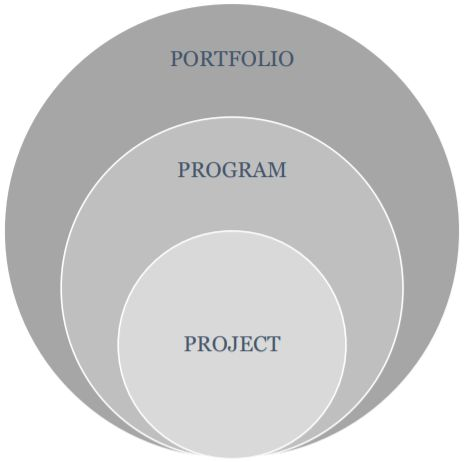
\includegraphics[width=3.5cm]{big_picture.jpg}
        \label{fig:bigpicture}
        \end{wrapfigure}
        \textbf{"Velký obrázek"}
        \begin{itemize}
            \item Portfolio je soubor projektů a programů řízených jako skupina k dosažení strategických cílů.
            \item Program je dočasný, závislý soubor projektů řízených jako skupina k dosažení společných cílů.
            \item Projekt dočasné úsilí o vytvoření jedinečného produktu, služby nebo výsledku.
        \end{itemize}
        \textbf{Portfolio} je pro naplnění strategických cílů a přidání hodnoty pro bussiness. Dosáhneme toho monitorováním výkonnosti bussinessu a prioritizováním a vybíráním projektů a programů.\\
        \textbf{Program} je pro koordinování a monitorování dané množiny projektů a pro dodání hodnot stakeholderům. Dosáhneme toho vyřešením omezení a konfliktů v projektech, přidělením rozsahu programu do projektů a managementem rizik programu.\\
        \textbf{Trojimperativ - čas, cena, rozsah -} definuje hranice projektu. Balancování trojimperativu je práce projektového managera. Redukce jedné strany zvyšuje tlak na zbylé dvě strany.\\
        \textbf{Management projektu začneme tak}, že přijmeme odpovídající standary, abychom získali lepší výsledky, efektivně koordinovali rozdílné aktivity, zvýšili transparentnost, důvěru u stakeholderů a vyhli se "vynálezu kola". Zde jsou nejpoužívanějši obecné standardy:
    \subsubsection{PRINCE2 - Projects in a Controlled Environment}
        Obecná metoda řízení projektu, předpisový přístup, Step-by-step vzorec pro úspěšný projekt.\\
        \textbf{7 principů} - Vůdčí povinnosti a best practises. Jejich přijetí nezaručí úspěch, ale vyhnutí jim zvýší šanci neúspěchu:
        \begin{itemize}
            \item Pokračující obchodní zdůvodnění - Jaké jsou důvody dělat projekt? Srovnejte tyto důvody s korporátní strategií a zdokumentujte je v Business case (obchodním případu).
            \item Poučte se ze zkušeností - uchovávejte si všechny naučené lekce. Nevynálézejte znovu kolo.
            \item Definované role a odpovědnosti - explicitně definujte strukturu týmu. Definujte a odsouhlaste role a odpovědnosti.
            \item Řiďte po etapách - přezkoumejte business case a plán po každé etapě. Hlašte senior managementu pro kontrolu. Vytvoří to zaměření a častý pocit úspěchu.
            \item Řiďte dle výjimek - Definujte odpovědnosti za cíle a toleranci pro čas, cenu, kvalitu, rozsah, riziko a přínosy. Odkazuj na překročené tolerance až na další úrovně managementu.
            \item Zaměřte se na produkty - Cíl není pracovat, ale vytvořit produkt.
            \item Přizpůsobení projektu - Nenásledujte PRINCE2 do posledního puntíku. Vyhněte se byrokracii nebo hrdinskému managementu.
        \end{itemize}
        \textbf{7 témat} - disciplíny projektu, které je třeba řešit neustále:
        \begin{itemize}
            \item Business case - Proč - rizika, časový rozsah, obchodní možnosti, očekávané benefity, disbenefity... Business zdůvodnění musí být validní během celého projektu.
            \item Organizace - Kdo - definice odpovědností. Identifikace 3 typů stakeholderů - business, uživatel, dodavatel. Přiřazení 3 stupňů management rolí - Project board, projektový manažer, týmový manažer. Řiď dle výjimek na vyšší level.
            \item Kvalita - Co - Vytvoř produkt, který dostojí očekávání. Monitoruj kvalitu plánů a reportů. Sepiš akceptující kritéria. Vytvoř strategii quality managementu.
            \item Plány - Jak, kolik, kdy - vytvoř plán projektu a plán etap. Plán pomocí Ganttova diagramu. Použij WBS jako páteř plánování.
            \item Riziko - Co když - buď proaktivní, identifikuj rizika a jejich pravděpodobnost a dopad, definuj odpověď na rizika.
            \item Změna - Jaký je dopad - Změny musí být v souladu s konfiguračním managementem. Zachyťte problémy. Zjistěte dopad změn, navrhněte možnosti.
            \item Pokrok - Kde jsme, kam jdeme, máme pokračovat - monitorujte a porovnávejte aktuální úspěchy vůči naplánovaným. Monitorujte čas, cenu a rozsah spolu s kvalitou, benefity a riziky.
        \end{itemize}
        \textbf{7 procesů} - průběh životního cyklu projektu. Od předprojektu až po uzavření projektu. Každý proces poskytujte množinu aktivit pro úspěšný projekt:
        \begin{itemize}
            \item Zahájení projektu - Přiřaďte klíčové lidi - Executive a projekt manager. Získejte zkušenosti od zkušených lidí. Připravte obrys business případu. Připravte project brief a plán další etapy. Získejte autorizaci od Project Boardu.
            \item Řízení projektu - Na konci každé etapy autorizuj plán pro další etapu, na konci projektu autorizuj ukočení projektu
            \item Iniciace projektu - Připrav management strategie pro rizika, konfigurace, kvalitu a komunikaci, připrav plán projektu, dokumentaci k zahájení projektu (PID) a upřesni business case.
            \item Kontrola etapy - Posuzuj pracovní balíčky, monitoruj etapy a zkoumej výjimky.
            \item Správa dodání produktu - Proces pro týmové managery, akceptuj, proveď a dodej pracovní balíčky.
            \item Správa mezí etapy - Plánuj další etapu, aktualizuj plán projektu a business case, hlášení konce etapy.
            \item Ukončení projetu - připrav plánované nebo předčasné ukončení, předej produkty, zhodnoť projekt.
        \end{itemize}
        PRINCE2 je nejlépe použitelný jako metoda pro následování od začátku projektu až po jeho ukončení. Je vhodný jak pro zkušené managery, tak i pro ty na základní úrovni.\\
        Zvažte PRINCE2, pokud firma potřebuje obsáhlá hlášení, kompletní projektovou dokumentaci a pokud tým potřebuje "rozkaž a kontroluj" typ managementu. Neobsahuje však požadavkový a rozpočtový management.
    \subsubsection{PMBOK - Project Management Body of Knowledge}
        Rozsáhlý průvodce osvědčenými postupy v managementu projektů. Je procesně orientovaný.\\
        \textbf{49 procesů} - každý proces je série aktivit s definovanými vstupy, výstupy, nástroji a technikami. Procesy jsou sdružené do 5 procesových skupin a 10 znalostních oblastí.\\
        \textbf{5 procesních skupin} - logické seskupení do procesů iniciace, plánování, provádění, monitorování a řízení a uzavírání.\\
        \textbf{10 znalostních oblastí} - disciplíny projektového managementu. Každá oblast má své definované procesy.
        \begin{itemize}
            \item Integrace - vytvoř (Project Charter) základní informace a základ pro využití zdrojů. Vytvoř plán projektového managementu.
            \item Rozsah - Získej požadavky, definuj, validuj a kontroluj rozsah. Vytvoř WBS.
            \item Plán - definuj a seřaď aktivity. Odhadněte trvání aktivit.
            \item Cena - Odhadněte cenu a rozpočet individuálních aktivit nebo pracovních balíčků na základě WBS. Kontrolujte ceny a rozpočet.
            \item Kvalita - Plánujte, řiďte a kontrolujte kvalitu
            \item Zdroje - Odhadněte fyzické a týmové zdroje všech aktivit. Získejte a kontrolujte zdroje. Vytvořte a řiďte tým.
            \item Komunikace - Plánujte, řiďte a monitorujte komunikace. Vytvořte, distribuujte a monitorujte informace o projektu.
            \item Riziko - identifikujte rizika, proveďte analýzu rizik, monitorujte rizika, plánujte a implementujte odpověď na rizika.
            \item Procurement - Kupte nebo získejte produkty nebo služby z vnějšku týmu. Kontrakty, nákupní objednávky, SLA... Vyberte prodávající a připravte kontrakty. Monitorujte výkon kontraktů.
            \item Stakeholdeři - Identifikujte je. Plánujte, řiďte a monitorujte jejich angažovanost na základě jejich potřeb.
        \end{itemize}
        Proces má definované vstupy, výstupy, nástroje a techniky.\\
        PMBOK je užitečný kdykoliv během projektu, je nejlépe užitý jako příručka, návod pro různé oblasti. Pro zkušeného i základního projektového managera.
        \begin{wrapfigure}{r}{0.25\textwidth}
        \centering
        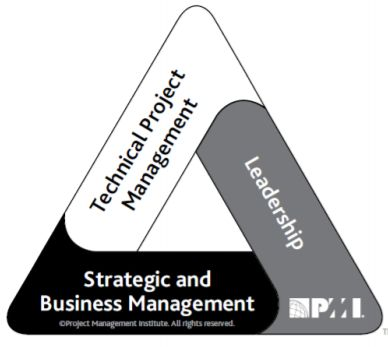
\includegraphics[width=3.5cm]{talent_triangle.jpg}
        \label{fig:talenttriangle}
        \end{wrapfigure}
        \textbf{Talentový trojúhelník} - technický projektový management (znalosti, dovednosti a chování ve vztahu k specifickým doménám projektového managementu), Leadership (... ve vztahu k řízení, motivování a směřování týmu), strategický a business management (znalosti a odbornost v průmyslu a organizaci).\\
        PMBOK může být užitečný kdykoliv během projektu. Nejlépe je použitelný jako příručka a návod pro různé oblasti znalostí. Je vhodný jak pro zkušené tak i pro základní projektové managery.
    \subsubsection{ICB - Individual Competence Baseline}
        Přístup založený na kompetencích.\\
        Individuální kompetence je aplikace znalostí, dovedností a schopností k dosažení požadovaného výsledku. Znalosti jsou kolekce informací a zkušeností. Dovednosti jsou specifické technické možnosti, které umožňují provádění úkolů. Schopnosti jsou efektivní poskytování znalostí a dovedností správným způsobem a ve správný čas.\\
        \textbf{5 perspektivních kompetencí}:
        \begin{multicols}{2}
        \begin{itemize}
            \item Strategie
            \item Řízení, struktury a procesy
            \item Dodržování, standardy a regulace
            \item Moc a zájem
            \item Kultura a hodnoty
        \end{itemize}
        \end{multicols}
        \textbf{13 kompetencí praxe}:
        \begin{multicols}{2}
        \begin{itemize}
            \item Návrh projektu
            \item Požadavky a cíle
            \item Rozsah
            \item Čas
            \item Organizace a informace
            \item Kvalita
            \item Finance
            \item Zdroje
            \item Procurement
            \item Plán a řízení
            \item Riziko a příležitost
            \item Stakeholders
            \item Změna a transformace
        \end{itemize}
        \end{multicols}
        \textbf{10 kompetencí lidí}:
        \begin{multicols}{2}
        \begin{itemize}
            \item Sebereflexe a sebeřízení
            \item Osobní integrita a spolehlivost
            \item Osobní komunikace
            \item Vztahy a angažovanost
            \item Leadership
            \item Týmová práce
            \item Konflikt a krize
            \item Vynalézavost
            \item Jednání
            \item Orientace výsledků
        \end{itemize}
        \end{multicols}
        ICB může být užitečný kdykoliv během projektu. Nejlépe je použitelný jako příručka na různé manažerské kompetence. Na rozdíl od ostatních standardů obsahuje velkou část o soft skillech. Je vhodný pro zkušené projektové managery.

    \subsection{2. přednáška \cite{pres-2}}
    \subsubsection{Projektový management v IT}
        \textbf{Specifika IT projektu}:
        \begin{itemize}
            \item Závislost projektů v portfoliu - neúspěch u jednoho projektu může mít kaskádový efekt u dalších.
            \item Potřeba managementu rizik - unikátnost, častá změna požadavků, nestabilní zdroje = vyšší riziko neúspěchu
        \end{itemize}
        \textbf{ITIL} - best practices pro management IT služeb. Pomáhá s otázkami co se stane před a po IT projektu. Má 5 etap životního cyklu:
        \begin{itemize}
            \item Strategie služeb - Jaká je strategie a poptávka po výstupu našeho projektu? Jakou službu vytváříme nebo podstatně měníme? Jak jsou finanční prostředky distribuovány v rámci služeb?
            \item Návrh služeb - Jaké jsou sazby SLA a dostupnost pro provoz naší služby? Jak zvládneme rizika na úrovni služeb? Jsou data a produkty v bezpečí a v souladu s obchodními politikami a právními požadavky?
            \item Přechod služeb - Jaké změny přináší náš projekt vůči existujícím službám? Jak nasazujeme náš software? Jak ukládáme a sdílíme znalosti získané během našeho projektu?
            \item Provoz služeb - Jakou dokumentaci poskytujeme pro helpdesk? Kdo bude řešit incidenty, požadavky a problémy? Jak spravujeme identity a přístup do našeho systému?
            \item Neustálé zlepšování služeb - Kdo bude sledovat, přezkoumávat, vyhodnocovat a aktualizovat naše služby, jakmile budou spuštěny?
        \end{itemize}
        \textbf{Typy IT projektů s příklady}
        \begin{itemize}
            \item Vývoj softwaru - Vytvoření interaktivní webové stránky
            \item IT procurement - Vybrání a nasazení nového antivirového programu
            \item IT síť a infrastruktura - Zlepšení zabezpečení sítě společnosti
            \item Systémová integrace - Nasazení aplikace WordPress, integrované s centralizovaným ověřováním a autorizací společnosti
        \end{itemize}
        \textbf{Vodopád} - jednoduchý a přímočarý, není flexibilní, obtížné splnit požadavky na změnu, nevhodné pro vývoj softwaru.\\
        \textbf{Spirála} - inkrementační (v každém inkrementu přidej něco nového), iterativní (návrh v opakovaných cyklech), vhodnější pro vývoj softwaru, většina SW vývojových frameworků je variací spirály.\\
        \textbf{Hlavní přístupy k vývoji SW}
        \begin{multicols}{2}
        \begin{itemize}
            \item Prediktivní
            \item Více pevnější
            \item Zaměření na procesy
            \item Pevné požadavky
            \item Důkladné plánování předem
            \item Například Unified Process
            \item Agilní
            \item Flexibilní a přizpůsobivý
            \item Zaměření na lidi
            \item Pravidelně aktualizované požadavky
            \item Minimální plánování předem
            \item Například SCRUM
        \end{itemize}
        \end{multicols}
    \subsubsection{Unified Process}
        Predktivní framework pro vývoj SW, iterativní a inkrementální přístup, řízen riziky a případy užití, architektonicky orientovaný.\\
        \textbf{Fáze životní cyklus UP}: začátek (inception), zpracování (elaboration), konstrukce (construction), přechod (transition).\\
        \begin{wrapfigure}{r}{0.5\textwidth}
        \centering
        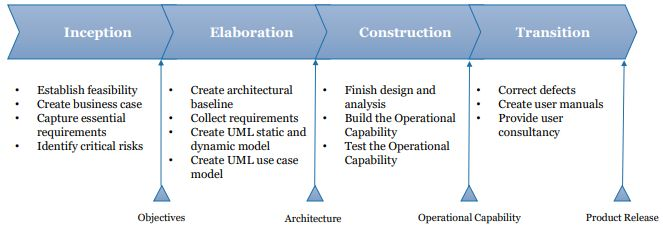
\includegraphics[width=10cm]{UP.jpg}
        \label{fig:UP}
        \end{wrapfigure}
        Každá iterace je jako malý projekt, neměla by trvat déle jak 3 měsíce. Rozdíl mezi dvěmi po sobě jdoucími iteracemi se nazývá inkrement. Iterace jsou shromažďovány do fází.\\
        \textbf{Každá iterace obsahuje 6 pracovních postupů}: business modelování (diagram aktivitú, požadavky (use case diagram), analýza a návrh (diagram tříd, sekvenční diagram), implementace (diagram tříd, diagram objektů), test (use case diagram, diagram tříd, diagram aktivit), nasazení (diagram nasazení).\\
    \subsubsection{SCRUM}
        Nejběžnější agilní framework pro vývoj SW. Jednoduchý pro porozumění, těžce zvládnutelný. Iterativní a inkrementální.
        \textbf{3 role}
        \begin{itemize}
            \item Vlastník produktu - reprezentuje stakeholdery, udržuje backlog produktu, hlavní odpovědností je komunikace
            \item SCRUM master - zaměřen na proces, odstraňuje překážky, hlavní odpovědností je řízení SCRUM procesu
            \item Tým developerů - 3 až 9 členů, organizovaný a sebeorganizovaný tým, udržují Sprint backlog, hlavní odpovědností je dodání produktu
        \end{itemize}
        \textbf{3 artefakty}
        \begin{itemize}
            \item Backlog produktu - Rozsah produktu, nezávislé položky ve formě User Stories. Vytváří jej celý SCRUM tým, vlastník produktu je za něj zodpovědný. Každá user story má vlastní Story Points připevněné k ní.
            \item Backlog sprintu - Podmnožina položek z backlogu produktu. Plán práce pro tento sprint. Udržován týmem developerů. Každá story je změněna na úkoly a daný odhad času pro tento úkol. Úkoly jsou rozděleny na To-Do, probíhající a splněné. Pořadí položek může být změněno. Položky nemůžou být přidány nebo odebrány (pouze při zrušení sprintu)
            \item Inkrement produktu - Součet všech položek backlogu produktu dokončených během sprintu, plus předchozí inkrementy. Vytvořen týmem developerů, testován uživateli, vydán vlastníkem produktu. Všechny úkoly sprint backlogu byly provedeny a inkrement musí být v použitelném stavu a splňuje definici hotového.
        \end{itemize}
        \textbf{5 událostí}
        \begin{itemize}
            \item Sprint - Iterace zaměřená na vývoj podmnožiny položek backlogu produktu. Podílí se na něm celý SCRUM tým. Vlastník komunikuje, developeři vyvíjí, SCRUM master řídí proces. Analyzuj - navrhni - vytvoř - testuj. Maximálně měsíc, všechny sprinty jsou stejně dlouhé. Končí použitelným inkrementem.
            \item Plánování sprintu - 8 hodinový meeting na ztačátku sprintu, celý SCRUM tým, nastavuje se cíl, vybírají se položky backlogu sprintu a přiřazují se k nim úkoly.
            \item Daily SCRUM - Každodenní 15 minutový meeting týmu developerů a možná i SCRUM mastera. Každý člen týmu odpoví na otázky: „Co jsem včera udělal?“, „Co dnes udělám?“, „Viděl jsem nějaké překážky?"
            \item Sprint review - 4 hodinový meeting celého SCRUM týmu a klíčových stakeholderů (zákazník). Zkontrolujte inkrement, backlog produktu a přepočítejte průběh projektu a datum dokončení.
            \item Retrospektiva - 3 hodinový meeting celého SCRUM týmu na konci sprintu. Prozkoumej vztahy mezi lidmi, procesy a nástroje během posledního sprintu. Co šlo dobře? Co můžeme zlepšit? Navrhni aspoň jedno zlepšení procesu do dalšího sprintu.
        \end{itemize}

    \subsection{3. přednáška \cite{pres-3b}}
    \subsubsection{Information System for disabled students part 1}
        \begin{multicols}{2}
        \begin{itemize}
            \item \textbf{S čím nám pomáhá IPMA a PMBOK?}
            \item Vytvoření projektové listiny
            \item Rozvoj klíčových strategií (komunikace, rizika, kvalita, změny)
            \item Osobní a mezilidské kompetence
            \item \textbf{S čím nám pomáhá SCRUM?}
            \item Vývojový proces
            \item Klíčové role, události a artefakty
            \item Neustálé zlepšování a integrace
        \end{itemize}
        \end{multicols}
        \textbf{12 principů agilního SW vývoje}
        \begin{itemize}
            \item Uspokoj zákazníka včasným a postupným dodáním
            \item Vítej měnící se požadavky, dokonce i pozdě ve vývoji.
            \item Dodávej fungující SW často
            \item Obchoďáci a developeři spolupracují denně
            \item Vybuduj projekty kolem motivovaných jednotlivců.
            \item Sděl informace prostřednictvím osobní konverzace.
            \item Funkční SW je primárním měřítkem pokroku
            \item Udržujte konstantní tempo na neurčito.
            \item Neustále věnujte pozornost technické dokonalosti
            \item Zjednodušte: maximalizujte množství dokončené práce.
            \item Podporuj samoorganizující se týmy.
            \item Podporuj retrospektivu týmů a ladění chování
        \end{itemize}
        \textbf{Agilní projektový manager} - tradiční role projektového managera je v agilních projektech distribuována napříč agilním týmem (tým vybírá úlohy, SCRUM máster s vlastníkem řeší problémy). PM volí spíše trenérský přístup než řídící.\\
        \textbf{Projektová listina} je dokument, který formálně autorizuje existenci projetu. Obsahuje:
        \begin{itemize}
            \item Business Case (Proč?) -  Odůvodnění projektu, klíčové rizika (dopady, plán reakce), souhrnné náklady (přímé - platy, licence, nepřímé - nájem vybavení), rozpočtování (cash flow a data fakturací) a očekávané benefity.
            \item Výsledek (Co?) - Popis produktu (očekávaný výsledek projektu), hlavní cíle a požadavky
            \item Stakeholdeři (Kdo?) - Externí a interní stakeholdeři. Externí budou interagovat a ovlivní celkový výsledek projektu, identifikuj jejich potřeby a angažovanost na projektu. Interní jsou součástí SCRUM týmu.
            \item Přístup (Jak?) -  použité standardy, očekávaný životní cyklus projektu, zvolené nástroje, metody, koncepty.
            \item Plán (Kdy?) - Hlavní milníky. Dobrým nástrojem je Ganntův diagram.
        \end{itemize}
        \textbf{Precedence Diagramming Method} je technika pro konstrukci rozvrhového modelu. Plánované aktivity se zobrazují jako posloupnost uzlů. Ty jsou graficky spojeny do jednoho či více logických vztahů: Finish-to-start (následující aktivita nemůže začít, dokud neskončí předchozí), Finish-to-finish (následující aktivita nemůže skončit, dokud neskončí předchozí), Start-to-start (následující aktivita nemůže začít, dokud nezačne předcházející), Start-to-finish (následující aktivita nemůže skončit, dokud nezačne předcházející). Může být součástí Ganttova diagramu.\\
        \textbf{Kontrakt} - mezi důležité dohody z perspektivy projektového managera patří: projektový přístup (očekávaná účast zákazníků), dohoda o platbě za čas a prostředky (člověkohodiny + materiál), minimální spotřeba práce, druh platby a platební podmínky.
    \subsection{4. přednáška}
    \subsubsection{Information System for disabled students part 2 \cite{pres-4a}}
        \textbf{Klíčové strategie managementu}
        \begin{itemize}
            \item Komunikace - K zajištění efektivní výměny informací
            \item Rizika - K zvládnutí nejistot, které by mohly ovlivnit výsledek projektu
            \item Změny - K definování procesu pro řízení změn u projektu
            \item Kvalita - K řízení kvality procesu a produktu
        \end{itemize}
        \textbf{Komunikační prvky v agilních principech}
        \begin{itemize}
            \item Osobní interakce - Pro lepší porozumění a získání okamžité odpovědi
            \item Jednoduchá dokumentace - Pro vyhnutí se byrokratickému managementu a podpůrné diskuze
            \item Ukaž, neříkej (Sprint review) - Shromáždi tým a stakeholdery.
            \item Rychlé mítinky - Pro podporu relevantní výměny informací.
        \end{itemize}
        \textbf{Prvky managementu rizik v agilních principech}
        \begin{itemize}
            \item Transparentnost a feedback - Pro vyhnutí nedorozumění v týmu
            \item Využití user stories a definice hotového - Pro vyjasnění
            \item Začlenění zákazníka do plánování a hodnocení - Aby se zabránilo nesprávným výkladům požadavků
            \item Krátké iterace - Pro snížení rizika spojená s rozpočtem a plánem
        \end{itemize}
        \textbf{Vývoj strategie rizik}
        \begin{itemize}
            \item Identifikuj rizika - na základě zkušeností z minulosti
            \item Posuď rizika - ohodnoť na základě pravděpodobnosti a dopadu. Definuj, jaké by byly následky.
            \item Definuj reakce na rizika - Akceptuj (neprováděj žádné akce, vypořádej se s rizikem, jakmile přijde), Vyhni se (změň plány pro vyhnutí se situaci), převeď (možný dopad na třetí stranu), sniž (sniž pravděpodobnost nebo dopad rizika.
            \item Specifikuj procesy monitorující rizika - Kdo je zodpovědný za monitorování rizik. Kde budou rizika definována. kdy budou rizika přezkoumána a aktualizována.
            \item Vytvoř registr rizik
        \end{itemize}
        \textbf{Dimenze SW rizik}
        \begin{itemize}
            \item Uživatel - nedostatek spolupráce, odpor vůči změnám
            \item Požadavky - měnící se požadavky, požadavky nedostatečně identifikovány
            \item Složitost projektu - použití nových technologií, vysoký úroveň technické složitosti
            \item Plánování a řízení - nezkušený projektový manažer
            \item Tým - nezkušení členové týmu
            \item Organizační prostředí - změny v managementu, nestabilní prostředí
        \end{itemize}
        \textbf{Nejčastější rizika SW vývoje} - pozdní požadavky na změnu, nedostatek personálu, nereálné odhady času a ceny, nedorozumění v požadavcích.\\
        \textbf{Prvky managementu změn v agilních (SCRUM) projektech} - Sprint review (přezkoumání projektu a diskutování možných změn backlogu produktu), častý feedback zákazníka, proaktivní reakce na změnu (předvídání změn v požadavcích).\\
        \textbf{Vývoj strategie managementu kvality}: 1. Nastav cíle kvality (dodej inkrement na čas s maximálně 2 \% defekty kódu), 2. Definuj opatření, která zlepšují kvalitu procesu (párové programování, přezkoumání kódu, retrospektiva sprintu), 3. Definuj opatření pro řízení, zajištění a kontrolu kvality produktu (testování jednotek, akceptační testování).\\
        \textbf{Zabudovaná opatření pro management kvality ve SCRUMu}:\\
        \textbf{Burndown graf} - zobrazuje zbývající práci pro daný časový úsek (Sprint nebo celý projekt). Zobrazuje, kolik hodnot už tým dodal a jak je blízko k dokončení závazku. Na osách jsou počet story pointů a počet dní sprintu.\\
        \textbf{Team velocity (rychlost týmu)} - kolik story pointů zvládne tým splnit během dne (sprintu). Pro předpovězení jak dlouho bude trvat dodání všech položek backlogu sprintu (produktu). Pomáhá pochopit kvalitu procesu - ideálně se časem rychlost týmu zvyšuje. Na osách je počet zbývajících story pointů a počet dní sprintu.\\
        \textbf{Definition of Done (definice hotového)} - vše, co je potřebné pro kompletaci inkrementu nebo backlogu produktu. Musí být pochopeno a sdíleno celým týmem. Pro pochopení, co je očekáváno od výstupů. Pro zajištění transparentnosti a kvality výstupů.\\
        Po potvrzení listiny projektu a klíčových strategií programovým managerem je v dalším kroku vytvořen backlog produktu a poté může začít první sprint.\\
        \textbf{Backlog produktu} je rozsah produktu. Nezávislé položky (funkce) ve formě user stories. Vytváří jej celý SCRUM tým, je za něj zodpovědný vlastník produktu. každá story má story pointy.\\
        \textbf{Tvorba backlogu produktu}:
        \begin{itemize}
            \item 1. Sestavte user stories (připojte akceptační kritéria, spojená rizika) - story je jasný popis funkce systému, agilní nástroj pro popis požadavků, obsahuje akceptační kritéria, může obsahovat spojená rizika.
            \item 2. Odhadněte user stories (čas, cena) - metrika jsou story pointy, reprezentují celkové úsilí týmu potřebné pro plnou implementaci user story, metoda odhadu je plánovací poker (každý z týmu dá jednotlivé story kartu odhadu - čas, který si myslí, že to zabere - a všechny karty se odhalí najednou. Diskutuje se, dokud se nedosáhne konsenzu.
            \item 3. Prioritizujte user stories - metoda MoSCoW (rozděl stories do kategorií - must have, should have, could have, won't have). Zvaž, jakou má story cenu pro zákazníka, jaké úsilí je třeba, množství odstraněného rizika.
        \end{itemize}
    \subsubsection{Information System for disabled students part 3 \cite{pres-4b}}
        \textbf{Plánování sprintu} - obecné informace viz přednáška 2.\\
        \textbf{Určení cíle sprintu} - cíl musí být viditelný (na Scrum tabuli), SMART (specifický, měřitelný, dosažitelný, relevantní, časově omezený), zahrnovat benefity podniknutí sprintu.\\
        \textbf{Vytvoření backlogu sprintu} - vyber položky z backlogu produktu, přiřaď úkoly k vybraným položkám, zobraz vše na SCRUM tabuli.\\
        \textbf{Daily SCRUM} - obecné informace viz přednáška 2.\\
        \textbf{pravidla Daily SCRUMu} - všichni by měli stát. Cokoliv, co někdo řekne, by mělo být užitečné a pochopitelné pro ostatní v místnosti. Striktně se držte plánu (začít včas, doba trvání 15 minut).\\
        \textbf{Sprinting} - během sprintu tým plní úkoly vyplynulé z user stories v backlogu sprintu. Čím více sprinty tým projde, tím lepší jsou v odhadování realizovatelného rozsahu.\\
        \textbf{Sprint review} - obecné informace viz přednáška 2.
        \begin{itemize}
            \item 1. Inspect increment - Vlastník produktu vysvětlí, které položky backlogu produktu byly dokončeny a které ne. Development tým diskutuje, co šlo dobře, jaké byly problémy a jak byly vyřešeny. Také předvede práce, kterou provedl. Následně odpovídá na otázky ohledně inkrementu.
            \item 2. Přezkoumání backlogu produktu - diskuze backlogu produktu tak, jak aktuálně je. Posouzení, co je nejcennější věcí, kterou je třeba udělat (možná změna pořadí položek backlogu). Upravte backlog produktu tak, aby vyhovoval novým příležitostem (přidání nových položek do backlogu).
            \item Výpočet pokroku projektu a data dokončení - přezkoumejte časovou osu, rozpočet a potencionální možnosti pro další předpokládané vydání.
        \end{itemize}
        \textbf{Sprint retrospective} - obecné informace viz přednáška 2. Zkontroluj a přízpůsob - lidi: pracoval někdo hůře? Zaslouží si někdo pochvalu? vztahy: vycházeli spolu lidi? Přivítal by někdo bližší spolupráci? procesy: Byl sprint dobře definován? nástroje: Používali jsme odpovídající komunikační nástroje?\\
    \subsection{5. přednáška}
    \subsubsection{Information System for disabled students part 4 \cite{pres-5}}
        \textbf{Řešení kofliktů v týmu} - Konflikty ničí dobré pracovní prostředí. Konflikty vyžadují rychlou reakci a zkušený úsudek. Konflikty někdy potřebuje nezávislého prostředníka. Konfliky mohou být ve stádiích: latentní (potencionální, ale zatím neviditelný), vznikající (viditelný, ale stále racionální) a eskalovaný (otevřený koflikt, neracionální).\\
        \textbf{De-eskalační techniky}
        \begin{multicols}{2}
        \begin{itemize}
            \item Snižte míru rozruchu, aby se diskuse stala možnou.
            \item Chovejte se klidně, i když nejste, je to stejně nakažlivé jako hněv nebo strach.
            \item Naslouchejte aktivně s empatií.
            \item Buďte zdvořilí, ne soudní.
            \item Pokud je to nutné, zkuste změnit téma na něco pozitivnějšího.
        \end{itemize}
        \end{multicols}
        \textbf{Požadavek na změnu} - Pokud má změna dramatický dopad na cíl sprintu, je sprint zrušen. Případně se po změně může stát, že se nějaká položka z backlogu produktu nedokončí nebo vůbec neimplementuje. Přidávání položek do backlogu produktu je vždy zodpovědností vlastníka produktu. Změní se registr rizik. Ve výjimečných případech se zvýší cena (pozdější doba dokončení nebo více zdrojů). Důležité je pokračovat s procesem, jak byl navržen.\\
        \textbf{Konečné vydání} - Konec vývoje je domluven na posledním Sprint review. Backlog produktu může ještě obsahovat nedokončené položky, ale tým společně se zákazníkem se shodli, že jsou nepotřebné. Na konci posledního sprintu je produkt považován za dokončený a plně vydaný.\\
        \textbf{Uživatelská dokumentace} - byla předávána průbězně. Zákazník dostává uživatelské dokumentace a instalační manuály. Ke konci sprintu pracujeme na user stories související s dokumentací. Pokud je třeba, je domluven trénovací meeting. Případně je předána i technická dokumentace, pokud nebyla domluvena podpora (po projektu). Podpora je domluvena v kontraktu. Uzavírají se zákaznické a dodavatelské kontrakty pro ujištění, že vše bylo splněno a význačné problémy byly vyřešeny.\\
        \textbf{Project retrospective} - způsob uzabření projektu s týmem. Pro přezkoumání dokončeného projektu a poučení se z úspěchů a neúspěchů. Přezkoumávají se reporty a časová osa včetně hlavních událostí a milníků. Odpovídá se a otázky: Co se mělo stát? Co se doopravdy stalo? Co jsme se naučili? Rekapitulují se osobní úspěchy a všem se děkuje. Je třeba skončit v pozitivním duchu.
    \subsection{6. přednáška}
    \subsubsection{SW solution for city information kiosks part 1 \cite{pres-6}}
        \begin{multicols}{2}
        \begin{itemize}
            \item \textbf{S čím nám pomáhá PRINCE2?}
            \item Terminologie
            \item Řídící principy
            \item Role
            \item Vypracování projektového plánu
            \item Reportování a projektová dokumentace
            \item \textbf{S čím nám pomáhá UP?}
            \item Vývojový proces produktu
            \item Analýza požadavků
            \item Produktová (technická) dokumentace
            \item
        \end{itemize}
        \end{multicols}
        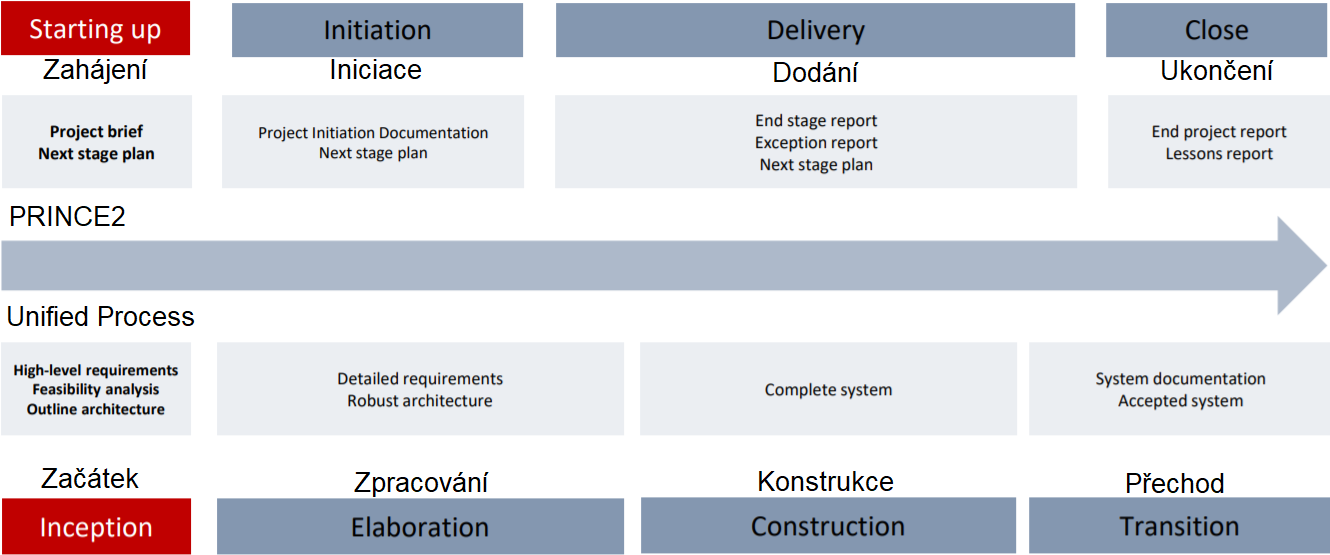
\includegraphics[width=\textwidth]{PRINCE2UP.png}
        \textbf{Fáze zahájení (začátek)}\\
        \begin{itemize}
            \item 1. Analyzuj vysokoúrovňové požadavky (UP)
            \begin{itemize}
                \item Urči vizi systému - společné chápání motivace pro budování systému. Vytvořeno společně se zákazníkem. Například: výhody poskytované aplikací. Problémy, které se vyřeší. Kdo jsou cíloví uživatelé.
                \item Popiš základní funkce systému - skrze: aktéry (popiš typického uživatele systému a klasifikuj je, identifikuj ostatní systémy, s kterými se bude interagovat) a případy užití (služby poskytované aktérům, v tomto případě pouze vysokoúrovňové funkce, může být ve formě Use Case diagramu nebo krátkého popisu)
            \end{itemize}
            \item Analytujte a zjistěte proveditelnost a obrys nastiňte obrys (UP) - stanovte aspoň jedno možné řešení. Vemte v potaz existující řešení, technologie nutné použít pro systém, jaké SW komponenty potřebujeme. Jaké jsou odhady nákladů, časového harmonogramu a souvisejících rizik?
            \item Project brief (PRINCE2) - Základní dokument, na základě kterého se Project Board rozhodně pokračovat. Ustanovení projektového management týmu včetně project boardu. Připraví se obrys business případu (zdůvodnění projektu, přehled nákladů, klíčové rizika...), zahrne se popis produktu a definuje se přístup k řízení (agilní vs. prediktivní).
            \begin{itemize}
                \item Součástí project boardu jsou: vedoucí (executive), seniorní uživatel, seniorní dodavatel, projektová manager, týmový manager.
                \item Definice přístupu k řízení - musí se zohlednit firemní nebo programové strategie, standardy projektového managementu, externí závislosti a prerekvizity projektu, technické možnosti životního cyklu vývoje produktu, vzdělávací potřeby uživatelů. Definovat by se mělo provozní prostředí, do kterého řešení musí zapadnout.
            \end{itemize}
            \item Plán další (initiation) fáze (PRINCE2) - Detailní každodenní plán. Referenční bod pokroku projektu. Vytvoří se Work Breakdown Structure (WBS), identifikují se aktivity a jejich závislosti, odhadne čas trvání aktivit a identifikují milníky, definují se role a zodpovědnosti a vytvoří se plán se vším předchozím (vizualizace v Ganttu nebo síťovém diagramu).
        \end{itemize}
    \subsection{7. přednáška}
    \subsubsection{SW solution for city information kiosks part 2 \cite{pres-7}}
        Momentálně jsme v Initiation/Elaboration fázi.\\
    \subsubsection{Project Initiation document (dokument o zahájení projektu)}
        Management produkt, který vždy odráží aktuální stav a plán projektu. Informace v projektu o Co, Proč, Kdo, Jak, Kde, Kdy, Jak moc... Odvozen z project brief a jednání se stakeholdery. Má význám pro definování projektu a vytvoření základů pro jeho řízení a hodnocení. Pro definování kontraktu mezi projektovým managerem a project board.\\
        Součásti Project Initation dokumentu: Detailní business případ, Struktura projektového managementu, Popis rolí, Přístup ke quality managementu, ke managementu změn, managementu rizik, managementu komunikace, projektový plán.\\
        \textbf{Detailní business případ} - Naším příkladem je zákazník/dodavatel projekt. Oba mají jejich vlastní business případ (důvod pro projekt). Zákazníkův je považován jako dominantní. Business případ je vlastněn vedoucím projektu. Obsahem business případu jsou: důvody pro projekt, očekávané benefity a tolerance, oceňování investic (zda mají smysl), harmonogram, náklady, hlavní rizika.\\
        \textbf{Struktura projektového managementu} - v project boardu sedí vedoucí, seniorní dodavatel, seniorní uživatel. Pod nimi je projektový manager a pod ním týmoví manageři. Project board reprezentuje klíčové kategorie stakeholderů, schvaluje hlavní plány, schvaluje výjimky a odchylky od plánu, komunikuje se stakeholdery.
        \textbf{Přístup ke quality managementu} - definování cílů kvality, definování strategie managementu kvality, vytvoření registru kvality, hledání schválení od project boardu.\\
        Registr kvality - událostí naplánovaných a realizovaných, udržuje se během projektu, poskytuje klíčové informace o auditu a ujištění.\\
        \textbf{Přístup k managementu změn} - definování základních linií produktu, definování, jak budou problémy zachyceny a vyhodnoceny, definování, jak budou opravné akce představeny a implementovány, vytvoření registru problémů.\\
        \textbf{Přístup k managementu rizik} - Identifikace a hodnocení rizik, plánování reakcí, plánování komunikace v managementu rizik, definování rolí a zodpovědností, vytvoření registru rizik\\
        \textbf{Přístup k managementu komunikace} - identifikace stakeholderů, definování komunikačních procedur.
    \subsubsection{Detailní analýza požadavků (UP)}
        \textbf{1. Sestavte podrobnosti většiny požadavků}\\
        \textbf{2. Vytvořte detailní případy užití na většině funkcí}\\
        \textbf{3. Vytvořte popis produktu} - detailní rozsah, součástí mockupy designu, základy pro smlouvu a ceny, co produkt musí dodat pro akceptování, rozdělení produktu do hlavních komponent.
    \subsubsection{Projektový plán}
        Součástí Project initiation dokumentu. Co, Proč, Kdo, Jak, Kde, Kdy, Jak moc informace celého projektu. Plán se aktualizuje na konci každé etapy.\\
        \textbf{Jak vytvořit Projektový plán}:
        \begin{itemize}
            \item 1. Vytvořte Work Breakdown Structure a určete pracovní balíčky - WBS je hieararchická dekompozice veškeré práce, kterou je potřebná udělat během plánu. Základ pro projektový harmonogram. Je to diagram neb hierarchický seznam všech výstupů a činností. Vytváří se podle specifikace produktu. Určtují se hlavní výstupy (systémy, subsystémy, komponenty) a rozdělují se do pracovních balíčků.
            \item 2. Vypočítejte odhady úsilí a nákladů pracovních balíčků - Pomocí PERTu, což je pravděpodobnostní technika pro odhad času potřebného k dokončení úkolu (aktivity, pracovního balíčku...). Úkol (pracovní balíček) má dány 3 typy času, které je třeba splnit, aby byl úkol splněn. Optimistický čas o (minimální možný), pesimistický čas p (maximální možný) a nejvíce pravděpodobný m (nejlepší odhad). Z těchto časů je vypočítán očekávaný čas te = (o + 4m + p) / 6.
            \item 3. Definování aktivit - závislosti mezi aktivitami, data začátku a konce a aktivit.
            \item 4. Přidělení zdrojů a zodpovědností - Matice přiřazení zdrojů ilustruje propojení mezi pracovními balíčky (aktivitami) a členy projektového týmu, může být vytvořena pro týmy i pro jednotlivce. Můžeme pomocí ní hledat všechny aktivity spojené s jednou osobou nebo všechny lidi spojené s danou aktivitou. Dále je zde RACI matice (Responsible, Accountable, Consult, Inform).
            \item Vytvořte plán s etapami a milníky projektu - CPM, Ganttův diagram.
        \end{itemize}
        \textbf{Critical Path Method (CPM)} - metoda pro stanovení nejdelšího úseku závislých aktivit v plánu. Komponenty: Seznam aktivit (pracovních balíčků), závislosti mezi aktivitami, logický začátek a konocové body. Pomocí tohoto se určuje, které aktivity jsou kritické (musí být dokončeny včas) a které mohou být zpožděny bez zpožďování projektu.
       \begin{center}
            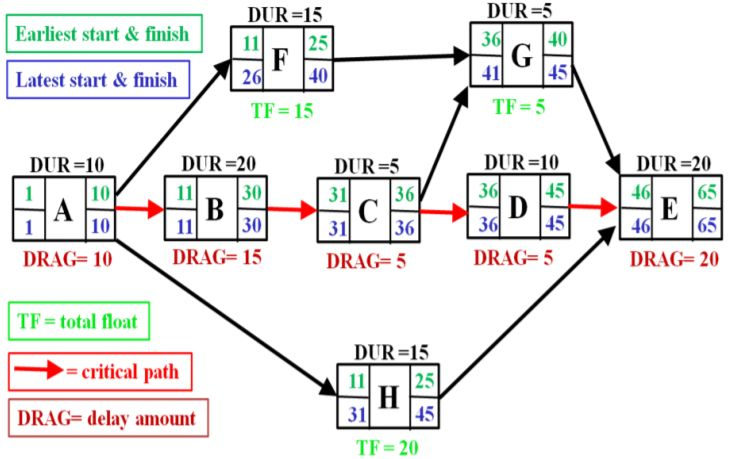
\includegraphics[width=0.5\textwidth]{CPM.jpg}
        \end{center}
        \textbf{Co se stane po sestavení PID?} - Používá se k získání oprávnění k pokračování projektu. Schváleno stakeholdery, project boardem. Je umístěn pod řízením změn. Bude použit pro porovnání plánovaného a aktuálního výkonu a pokroku. Je k dispozici všem, kteří se podílejí na projektu pro poradenství a informace.\\
        \textbf{Zpráva o konci etapy} dává přehled o pokroku a celkové situaci projektu. Dává základ project boardu pro rozhodování, co dál dělat s projektem. Obsahuje posudek, jak si projekt stojí v porovnání s plány, posudek o výkonu týmu a posudek o produktu (součástí i záznamy o kvalitě).\\
        \textbf{Plán další (dodání) etapy} je detailní každodenní plán pro další etapu (asi 3 měsíce dlouhá). Referenční bod pokroku pokroku projektu. Vytváří se pomocí kroků z "Jak vytvořit projektový plán".
    \subsection{8. přednáška}
    \subsubsection{SW solution for city information kiosks part 3 \cite{pres-8}}
        Momentálně jsme v Delivery/Elaboration a Construction fázi.\\
        \textbf{Robustní architektura (UP)} - kostra systému, základ, na kterém se implementuje zbytek systému. Zabýváme se otázkou, zda je třeba vše postavit znovu nebo zda můžeme něco znovu použít nebo koupit. Popis, jak subsystémy a klíčové komponenty budou spolupracovat. Implementace a testování nejdůležitějších scénářů. Díky RB lépe porozumíme systému, vyřešíme všechny hlavní technické rizika, odpovídajícím způsobem naplánujeme projekt.\\
        \textbf{Organizování týmů kolem architektury} - osobní komunikace se nestupňuje dobře. Organizace kolem architektury minimalizuje příliš mnoho komunikace. Architektonický tým řeší problém vždy s týmem, který má na starost implementaci subsystému s daným problémem.\\
        \textbf{Delivery (dodací) fáze (PRINCE2)} je složena obvykle z několika etap (iterací), kde každá dáze je jako mini-projekt a neměl by trvat déle než 3 měsíce. Projektový manažer má jako hlavní zodpovědnost udržet projekt v mezích času, nákladů, rozsahu a kvality.\\
        \textbf{Procesy Delivery etapy}: Kontrolování etapy, management dodávání produktu, management hranic etapy.\\
        \textbf{Kontrolování etapy} - zodpovědností projektového managera je autorizování, přijímání a přezkoumání pracovních balíčků, používání reportů ke správě pokroku, management rizik a problémů.\\
        Výstupy jsou: pracovní balíčky, Highlights report, denní záznamy, aktualizace registrů chyb a rizik.\\
        Pracovní balíček je množina informací relevantních ro výrobu jednoho či více produktů. Obsahuje popis práce a produktů. Používá se pro rozdělená práce do balíčků, které mohou být monitorovány a sestaveny s ohledem na kvalitu, náklady a čas.\\
        Highlights report - Souhrnný přehled o stavu etapy. Informace o průběhu pracovních balíčků, nový rizicích a problémech. Pomocí něj se poskytuje informace o stavu etapy Project Boardu.\\
        Eskalující problémy a rizika - Když problém nebo riziko přesáhne toleranci domluvenou s project board, informujte jej a vytvořte Exception report (důsledky problému nebo rizika, doporučení).\\
        \textbf{Management dodávání produktu} - zobrazuje projekt z pohledu týmového managera. Kontrolování etapy zobrazuje projekt z pohledu projektového managera. Zodpovědností týmového managera je produkovat týmový plán, demonstrovat kvalitu produktu, přijmout, provést a doručit pracovní balíčky.\\
        Výstupy jsou: Týmový plán a pracovní balíček.\\
        Týmový plán je volitelná úroveň plánu použitého pro konkrétní tým. Obsahuje členění činností v rámci pracovních balíčků zahrnutým v týmovém plánu. Definuje začátek a konec činností, přiřazuje zdroje a definuje milníky. Používá se pro kontrolu dodání pracovník balíčků během etapy.\\
        \textbf{Management hranic etapy} - Zodpovědností projektového managera je přezkoumat aktuální etapu, plán po další etapu, aktualizovat PID.\\
        Výstupy jsou: zpráva o konci etapy, plán další etapy, aktualizace projektového plánu, registrů rizik, problémů a kvalit, business případu.\\
        Zpráva o konci etapy je stejná jako v předchozí přednášce.\\
        Plán další (delivery) fáze je stejný jako v předchozí přednášce.
    \subsection{9. přednáška}
    \subsubsection{SW solution for city information kiosks part 4 \cite{pres-9a}}
        Momentálně jsme v close/Transition fázi.\\
        \textbf{Konec konstrukce (UP)} - fáze z Unified Process, v poslední fázi Constructionu máme k dispozici Beta systém, který je přiměřeně stabilní, integrovaný, testovaý a k dispozici pro použití.\\
        \textbf{Přechodová fáze (UP)} - zbývá nám v této poslední fázi Unified Process udělat, aby byl systém akceptován:
        \begin{itemize}
            \item Beta testování - získáváme feedback od beta testerů, feedback jsou požadavky na změny (oprava bugů, malé úpravy systému)
            \item Dokumentace a trénování - uživatelská dokumentace je návod, jak používat systém. Operační manuál je návod, jak spustit systém. Trénovací materiály jsou praktické kurzy a workshopové schůze.
            \item Akceptační testování - formální testování systému, finální verifikace požadované funkcionality, zda požadavky v kontraktu byly splněny. Procedura zahrnuje sepisování akceptačních protokolů.
        \end{itemize}
        \textbf{Ukončovací fáze (PRINCE2)} obsahuje:
        \begin{itemize}
            \item Předání produktu - doporučení pro následné činnosti, definuje se a domlouvá se podpora produktu, zajišťuje se SLA o podpoře (ceny, servisní doba, reakční doba, penalizace, SLA pokryto ITILem), získává se akceptační protokol, přesouvá se zodpovědnost z projektu na provoz a údržbu.
            \item Zprává o ukončení projektu - formálně ukončí práci na projektu. součástí je shrnutí projektového managera o výsledku projektu, přezkoumání business případu, dosažené přínosy, výkonnost týmu a produktů. Toto shrnutí se poskytuje i stakeholderům, posuzuje se z něj i úspěšnost projektu.
            \item Lessons report (zpráva o lekcích) - Vyjmenovává zkušenosti a znalosti, které by mohly zlepšit budoucí projekty. Jsou v tom doporučení pro korporátní a programový management, hodnocení metod projektového managementu, úvaha zákazníka, abnormální události a jejich příčiny a doporučení.
        \end{itemize}
\section{Fulltext otázky}
    Tyto otázky nejsou z minulých let, jedná se pouze o můj tip, jaké fulltextové otázky by se mohly objevit. Rozhodně se můžou objevit otázky na výhody a nevýhody jednotlivých standardů (UP, PRINCE2, ...) a přístupů k SW developmentu (agilní, prediktivní) nebo na shodné a rozdílné prvky dvou standardů nebo přístupů k SW developmentu.

    \begin{minipage}{\textwidth}
        \textbf{ \mypara Kdy použít Unified Process?}\\
        Jako prediktivní, bez překvapení proces když je většina požadavků známá, když potřebujete potřeba kompletní kontrola nad procesem a týmem, když vývojový proces potřebuje podrobnou dokumentaci (UML diagramy).\\
     \end{minipage}

    \begin{minipage}{\textwidth}
        \textbf{ \mypara Výhody a nevýhody Unified Processu (prediktivního DP)?}\\
        \begin{multicols}{2}
        \begin{itemize}
            \item \textbf{Výhody}
            \item Zákazník dostane definici produktu v kontraktu
            \item Není potřeba dozoru zákazníka během projektu
            \item
            \item
            \item \textbf{Nevýhody}
            \item Striktní deadliny
            \item Plnění požadavků na změnu je těžké
            \item Projekt potřebuje více času na plánování
            \item Kontrakt musí obsahovat více specifik
        \end{itemize}
        \end{multicols}
     \end{minipage}

     \begin{minipage}{\textwidth}
        \textbf{ \mypara Kdy použít SCRUM?}\\
        Jako adaptivní framework, když nejsou k dispozici přesné požadavky, tým je silný v komunikaci a spolupráci, zákazník chce alespoň část produktu co nejdříve.\\
     \end{minipage}

     \begin{minipage}{\textwidth}
        \textbf{ \mypara Výhody a nevýhody SCRUMu?}\\
        \begin{multicols}{2}
        \begin{itemize}
            \item \textbf{Výhody}
            \item Flexibilní kontrakt
            \item Rozsah není hned znám, můžeme jednoduše přidávat funkce a splnit požadavky na změnu
            \item Častější dohled zákazníka dodává více důvěry
            \item \textbf{Nevýhody}
            \item Konstantní spolupráce se zákazníkem vyžaduje čas navíc
            \item Těžké předpovědět finální rozpočet a deadline
            \item Řízení trojimperativu se stává nepřetržitým úkolem
        \end{itemize}
        \end{multicols}
     \end{minipage}

     \begin{minipage}{\textwidth}
        \textbf{ \mypara Kdy je PRINCE2 vhodný?}\\
        \begin{multicols}{2}
        \begin{itemize}
            \item Projektový manager potřebuje následovat obsáhlou metodu
            \item Projektový manager má málo zkušeností
            \item Kultura společnosti vyžaduje obsáhlé reportování
            \item Projekt musí být důkladně zdokumentován
            \item Tým potřebuje management typu "vel a kontroluj"
            \item Tým je velký a rozmanitý
            \item Není třeba managementu založeného na silném vedení
        \end{itemize}
        \end{multicols}
    \end{minipage}

    \begin{minipage}{\textwidth}
        \textbf{ \mypara Kdy není PRINCE2 vhodný?}\\
        \begin{multicols}{2}
        \begin{itemize}
            \item Byrokratické přetížení není vítané
            \item Požadavky na změnu musí být splněny okamžitě
            \item Rozhodování je odpovědností celého týmu
        \end{itemize}
        \end{multicols}
    \end{minipage}

    \begin{minipage}{\textwidth}
        \textbf{ \mypara Kdy je PMBOK vhodný?}\\
        \begin{multicols}{2}
        \begin{itemize}
            \item Projektový manažer potřebuje podrobnosti o tom, jaké nástroje a techniky použít pro klíčové oblasti znalostí projektu
            \item Zaměřujeme se na procesy a postupy
        \end{itemize}
        \end{multicols}
    \end{minipage}

    \begin{minipage}{\textwidth}
        \textbf{ \mypara Kdy není PMBOK vhodný?}\\
        \begin{multicols}{2}
        \begin{itemize}
            \item Projektový manager potřebuje následovat obsáhlou metodu
            \item Projekt vyžaduje časté adresování soft skill nástrojů a technik.
        \end{itemize}
        \end{multicols}
    \end{minipage}

    \begin{minipage}{\textwidth}
        \textbf{ \mypara Kdy je ICB vhodný?}\\
        \begin{multicols}{2}
        \begin{itemize}
            \item Pro projekt je klíčové využití soft skills (např. Komunikace, leadership, řešení konfliktů a krizí)
            \item Kompetence projektového manažera vyžadují častou pozornost a hodnocení
            \item Projektový manažer má zkušenosti s dobrým porozuměním projektových procesů a znalostních oblastí
        \end{itemize}
        \end{multicols}
    \end{minipage}

    \begin{minipage}{\textwidth}
        \textbf{ \mypara Kdy není ICB vhodný?}\\
        \begin{multicols}{2}
        \begin{itemize}
            \item Projektový manager potřebuje následovat obsáhlou metodu
            \item Projektový manager má málo zkušeností
            \item Kultura společnosti vyžaduje obsáhlé reportování
        \end{itemize}
        \end{multicols}
    \end{minipage}

    \begin{minipage}{\textwidth}
        \textbf{ \mypara Kdy je UP vhodný?}\\
        \begin{multicols}{2}
        \begin{itemize}
            \item Požadavky jsou jasné, stabilní a známé předem
            \item Projekt je rozsáhlý a heterogenní
            \item Projekt vyžaduje důkladné včasné etapové plánování
            \item Společnost nebo zákazník vyžaduje důkladnou dokumentaci
        \end{itemize}
        \end{multicols}
    \end{minipage}

    \begin{minipage}{\textwidth}
        \textbf{ \mypara Kdy není UP vhodný?}\\
        \begin{multicols}{2}
        \begin{itemize}
            \item Očekávají se časté požadavky na změnu
            \item Tým projektu potřebuje svobodu a flexibilitu
        \end{itemize}
        \end{multicols}
    \end{minipage}

    \begin{minipage}{\textwidth}
        \textbf{ \mypara Kdy je SCRUM vhodný?}\\
        \begin{multicols}{2}
        \begin{itemize}
            \item Přesné požadavky nejsou předem známy
            \item Klíčovým faktorem je čas na trhu (rychlost dodávání výsledků)
            \item Rychlá zpětná vazba zúčastněných stran je zásadní
            \item Vedený tým je silný ve spolupráci a otevřené komunikaci
            \item Projekt má průzkumný nebo inovační charakter
            \item Pracovní problém je složitý a nelze ho přizpůsobit redukcionismu
        \end{itemize}
        \end{multicols}
    \end{minipage}

    \begin{minipage}{\textwidth}
        \textbf{ \mypara Kdy není SCRUM vhodný?}\\
        \begin{multicols}{2}
        \begin{itemize}
            \item Vedený tým není disciplinovaný, motivovaný a ochotný tvrdě pracovat
            \item Vedený tým je větší než 15 osob
            \item Vedený tým je distribuován na různých místech
            \item Projekt je z hlediska bezpečnosti kritický
            \item Zajištění kvality musí být zaměřeno na procesy
            \item Rozsah projektu je velký a heterogenní
        \end{itemize}
        \end{multicols}
    \end{minipage}

    \begin{minipage}{\textwidth}
        \textbf{ \mypara S čím standardy projektového managementu pomůžou a s čím ne?}\\
        \begin{multicols}{2}
        \begin{itemize}
            \item \textbf{Pomůžou s}
            \item Netechnickými aspekty projektu
            \item Managementem stakeholderů
            \item Managementem rizik
            \item \textbf{Nepomůžou s}
            \item Správou požadavků
            \item Používáním developmentu procesu
            \item Testováním
        \end{itemize}
        \end{multicols}
    \end{minipage}

    \begin{minipage}{\textwidth}
        \textbf{ \mypara Jak vybrat vhodné standardy pro váš projekt?}\\
        \begin{itemize}
            \item Znát výhody a omezení každého standardu
            \item Zkontrolujte profil, kulturu a zásady vaší společnosti a společnosti zákazníka
            \item Otestujte zkušenosti projektového týmu, dovednosti a spolupráci
            \item Přezkoumejte oblasti projektu, rozsah a požadavky
            \item Vyberte si standard nebo kombinaci standardů, které jsou v souladu s danými podmínkami
        \end{itemize}
     \end{minipage}

    \begin{minipage}{\textwidth}
        \textbf{ \mypara Vysvětlete projekt, program, portfolio.}\\
        \textbf{Projekt} - unikátní, proveden jednou, naplánovaný, řízení projektu znamená udržet věci na správné cestě, nejlépe vizualizován Ganntovým diagramem, může být složen z unikátního souboru procesů, které lze opakovat a automatizovat. Je spojen s riziky, má deadliny, přinášíme změnu, děláme něco nového.\\
        \textbf{Program} - je pro koordinování a monitorování dané množiny projektů a pro dodání hodnot stakeholderům. Dosáhneme toho vyřešením omezení a konfliktů v projektech, přidělením rozsahu programu do projektů a managementem rizik programu.\\
        \textbf{Portfolio} - je pro naplnění strategických cílů a přidání hodnoty pro bussiness. Dosáhneme toho monitorováním výkonnosti bussinessu a prioritizováním a vybíráním projektů a programů.
     \end{minipage}

     \begin{minipage}{\textwidth}
        \textbf{ \mypara Uveďte 2 rozdílné a 3 shodné prvky ICB a PRINCE2 certifikací.}\\
        \begin{multicols}{2}
        \begin{itemize}
            \item \textbf{2 rozdíly}
            \item PRINCE2 je vhodný pro nezkušené projektové managery
            \item ICB má přístup založen na kompetencích, PRINCE2 předpisový
            \item \textbf{3 shody}
            \item Oba frameworky jsou vhodné pro zkušené PM
            \item Možnost certifikace projektového manažera zkouškou
            \item Zabývají se stejnými věcmi, například: rizika, kvalita, stakeholdeři, požadavky na změnu, management rizik
        \end{itemize}
        \end{multicols}
     \end{minipage}

     \begin{minipage}{\textwidth}
        \textbf{ \mypara Co se použije ze SCRUM a IPMA na agilním projektu?}\\
        \begin{itemize}
            \item (IPMA) Základní projektová dokumentace
            \item (IPMA) Přístupy k rížení rizik, kvality a změny
            \item (IPMA) Osobní kompetence
            \item (SCRUM) Vývojový proces
            \item (SCRUM) Klíčové role, události, artefakty
        \end{itemize}
     \end{minipage}

     \begin{minipage}{\textwidth}
        \textbf{ \mypara Co se použije z PRINCE2 a UP na prediktivním projektu?}\\
        \begin{itemize}
            \item (UP) Proces developmentu produktu
            \item (UP) Analýza požadavků
            \item (PRINCE2) Technická dokumentace
            \item (PRINCE2) Terminologie a řídící zásay
            \item (PRINCE2) Plánování, reportování a projektová dokumentace
        \end{itemize}
     \end{minipage}

     \begin{minipage}{\textwidth}
        \textbf{ \mypara Jaké jsou rozdíly mezi agilním a prediktivním projektem z hlediska týmu?}\\
        \begin{multicols}{2}
        \begin{itemize}
            \item \textbf{Agilní projekt}
            \item Malý tým, na jednom místě, motivovaný
            \item Osobní komunikace
            \item Spolupráce na základě důvery a znalostí
            \item Časté krátké mítinky, které podporují transparentnost
            \item Sebeorganizovaný tým (zodpovědnosti developera se mohou hýbat)
            \item \textbf{Prediktivní projekt}
            \item Velký a různě rozmístěný tým
            \item Centrální architektický tým jako integrační bod komunikace
            \item Komunikace více formální napříč týmy
            \item Reporty jako základní způsob komunikace
            \item Jasné, formální vymezení rolí a odpovědností
        \end{itemize}
        \end{multicols}
    \end{minipage}

    \begin{minipage}{\textwidth}
        \textbf{ \mypara Jaké jsou rozdíly mezi agilním a prediktivním projektem z hlediska zákazníka?}\\
        \begin{multicols}{2}
        \begin{itemize}
            \item \textbf{Agilní projekt}
            \item Například projekt IS pro centrum pro postižené studenty
            \item Zákazník více zaměřen na pomoc studentům než na profit a přísné deadliny
            \item Požadována pouze základní dokumentace
            \item Časté zapojení zákazníka a zpětná vazba
            \item Spokojenost zákazníka založená na řešení aktuálních potřeb
            \item \textbf{Prediktivní projekt}
            \item Lokální vládní instituce s přísnou politikou
            \item Striktní deadliny a rozpočet
            \item Vyžaduje detailní specifikace před ukončením
            \item Menší potřeba dohledu zákazníka během projektu
            \item Spokojenost zákazníka založená na doručení toho, co bylo definováno předem
        \end{itemize}
        \end{multicols}
    \end{minipage}

    \begin{minipage}{\textwidth}
        \textbf{ \mypara Jaké jsou rozdíly mezi agilním a prediktivním projektem z hlediska projektu?}\\
        \begin{multicols}{2}
        \begin{itemize}
            \item \textbf{Agilní projekt}
            \item Krátce trvající projekt
            \item Rychlé dodávání výsledků
            \item Nepředvídatelný rozsah
            \item Čas a cena jsou fixní, rozsah je flexibilní, záleží na aktuální potřebě zákazníka
            \item Změny se musí dít bez větší námahy\\ \\ \\
            \item \textbf{Prediktivní projekt}
            \item Projekt s velkým a různorodým rozsahem a dlouhým trváním
            \item Výsledky nejsou očekávány dříve než na konci projektu
            \item Kontrola a koordinace prostřednictvím monitorování a reportů
            \item Rozsah, čas a cena jsou více fixované a definované předem
            \item Důraz na následování plánu, změny jsou jasně zdokumentovány
        \end{itemize}
        \end{multicols}
    \end{minipage}

    \begin{minipage}{\textwidth}
        \textbf{ \mypara Jaké jsou rozdíly mezi agilním a prediktivním projektem z hlediska životního cyklu projektu?}\\
        \begin{multicols}{2}
        \begin{itemize}
            \item \textbf{Agilní projekt}
            \item Krátké počáteční plánování s definovanými klíčovými strategiemi
            \item Backlog produktu je v centru plánování a hodnocení projektu
            \item Vývoj v krátkých iteracích o stejné časové délce (Sprint)
            \item Inkrementy uvolněné na konci každého sprintu
            \item Uzavření (Closing) projektu je příležitostí k zdokonalení řešení a poučení z chyb
            \item \textbf{Prediktivní projekt}
            \item Důkladná iniciační fáze s důrazem na plánování
            \item PID je v centru plánování a hodnocení projektu
            \item Vývoj v iteracích o délce 3 měsíců
            \item Částečná integrace systému na konci každé iterace
            \item Přechodná (Transition) fáze zahrnuje hlavní release produktu a akceptační testování
        \end{itemize}
        \end{multicols}
    \end{minipage}

    \begin{minipage}{\textwidth}
        \textbf{ \mypara Jaké jsou rozdíly mezi agilním a prediktivním projektem z hlediska rizik a kvality?}\\
        \begin{multicols}{2}
        \begin{itemize}
            \item \textbf{Agilní projekt}
            \item Transparentnost a stálá zpětná vazba jako implicitní strategie rizik
            \item Krátké iterace snižují rizika spojená s rozpočtem a plánem
            \item Méně rizik spojených s měnícími se požadavky. Hlavními zdroji rizik jsou nové technologie a závislosti
            \item Důraz na retrospektivy a poučení z chyb
            \item Kvalita orientovaná na zákazníka. Základním ukazatelem kvality je spokojenost zákazníků
            \item \textbf{Prediktivní projekt}
            \item Přístup orientovaný na architekturu řeší hlavní technická rizika na počátku developmentu procesu
            \item Více rizik souvisí s počátečním odhadem nákladů a zdrojů
            \item Formální dokumentace problémů a jejich řešení
            \item Kvalita formálně přezkoumána prostřednictvím registru kvality
            \item Kvalita orientovaná na procesy. Hlavním ukazatelem kvality je dodržování počátečních požadavků a plánu
        \end{itemize}
        \end{multicols}
    \end{minipage}

\newpage

\section{Literatura}

    \bibliographystyle{czechiso}
    \begin{flushleft}
        \bibliography{quotation}
    \end{flushleft}


\end{document}
